\begin{enumerate}
\def\labelenumi{\arabic{enumi})}
\setcounter{enumi}{22}
\tightlist
\item
  Let \((\mathrm{W},\mathrm{S})\) be a Coxeter system and \(k\) a commutative ring. Suppose that we are given, for all \(s\in S\) , two elements \(\lambda_{s}\) and \(\mu_s\) of \(k\) such that \(\lambda_{s} = \lambda_{s'}\) and \(\mu_{s} = \mu_{s'}\) whenever \(s\) and \(s'\) are conjugate in W. Put \(\mathbf{E} = k^{(\mathbf{W})}\) and let \(\{e_w\}\) be the canonical basis of E.
\end{enumerate}

\begin{enumerate}
\def\labelenumi{\alph{enumi})}
\tightlist
\item
  Show that \(E\) has a unique algebra structure such that, for \(s \in S\) and \(w \in W\) ,
\end{enumerate}

\[
e _ {s}. e _ {w} = \left\{ \begin{array}{l l} e _ {s w} & \text {if} l (s w) > l (w) \\ \lambda_ {s} e _ {w} + \mu_ {s} e _ {s w} & \text {if} l (s w) <   l (w) \end{array} \right.
\]

(introduce the endomorphism \(P_{s}\) of E defined by the above formulas, where \(e_{s}.e_{w}\) is replaced by \(\mathrm{P}_{s}(w)\) , and the endomorphism \(Q_{s}=jP_{s}j^{-1}\) , where j denotes the automorphism of E defined by \(j(e_{w})=e_{w^{-1}}\) ; show that \(P_{s}Q_{t}=Q_{t}P_{s}\) for \(s,t\in S\) by remarking that the conditions \(l(swt)=l(w)\) and \(l(sw)=l(wt)\) imply that sw=wt; then argue as in Exerc. 3 c)). The module E, equipped with this algebra structure, will be denoted by \(\mathrm{E}_{k}((\lambda_{s}),(\mu_{s}))\) . Show that \(\mathrm{E}((0),(1))\) is the group algebra k{[}W{]} of W (Algebra, Chap. III, §2, no. 6).

b) Show that the family of generators \((e_s)_{s\in S}\) and the relations

\[
e _ {s} ^ {2} = \lambda_ {s} e _ {s} + \mu_ {s} \mathrm{for} s \in S
\]

\((e_s e_t)^r = (e_t e_s)^r\) for \(s, t \in S\) such that \(st\) is of finite even order \(2r\) \((e_s e_t)^r e_s = (e_t e_s)^r e_t\) for \(s, t \in S\) such that \(st\) is of finite odd order \(2r + 1\)

form a presentation of the algebra \(\mathbf{E}\) (argue as in the proof of Th. 1 of no. 6 of §1).

\begin{enumerate}
\def\labelenumi{\arabic{enumi})}
\setcounter{enumi}{23}
\tightlist
\item
  Let G be a group and B a Tits subgroup of G (Exerc. 3, of which we use the notation). Assume that, for all \(s \in S\) , the double coset \(C(s)\) is the union of a finite number \(q_{s}\) of left cosets with respect to B. We use the notation of Exerc. 22 and put \(a_{w} = a_{\mathrm{C}(w)}\) for all \(w \in W\) .
\end{enumerate}

\begin{enumerate}
\def\labelenumi{\alph{enumi})}
\item
  Show that conditions (i) and (ii) of Exerc. 22 are satisfied. We can therefore speak of the Hecke algebra \(\mathrm{H}_k(\mathbf{G},\mathbf{B})\) ( \(k\) being a commutative ring), of which \((a_w)_{w\in \mathbb{W}}\) is a basis.
\item
  Let \(s \in S\) and \(w \in W\) . Show that \(a_s * a_s = (q_s - 1)a_s + q_s\) ; show that if \(l(sw) > l(w)\) then \(a_s * a_w = a_{sw}\) .
\item
  Show that the linear map from the algebra \(\mathrm{E}_{k}((q_{s}-1),(q_{s}))\) associated to the Coxeter system (W,S) (Exerc. 23) to \(\mathrm{H}_{k}(\mathrm{G},\mathrm{B})\) that sends \(e_{w}\) to \(a_{w}\) for all \(w \in W\) is an isomorphism of algebras.
\end{enumerate}

\begin{enumerate}
\def\labelenumi{\arabic{enumi})}
\setcounter{enumi}{24}
\tightlist
\item
  We use the notation of Exerc. 8. Assume in addition that, for all \(s \in S\) , the index \(q_s\) of \(B \cap gBg^{-1}\) in \(B\) is finite for all \(g \in BsB\) .
\end{enumerate}

\begin{enumerate}
\def\labelenumi{\alph{enumi})}
\item
  Show that the pair \((\tilde{\mathbf{G}},\mathbf{B})\) satisfies conditions (i) and (ii) of Exerc. 22.
\item
  Show that, for all \(\gamma \in \Gamma\) , the map \(x \mapsto \gamma x \gamma^{-1}\) defines an automorphism \(\sigma\) of the Hecke algebra \(\mathrm{H}_k(\mathrm{G}, \mathrm{B})\) and that \(\sigma\) depends only on the class \(\omega\) of \(\gamma\) in \(\Omega = \Gamma / (\Gamma \cap \mathrm{B})\) .
\item
  Let \(k[\Omega]\) be the group algebra of \(\Omega\) and \((e_{\omega})\) its canonical basis. Show that the linear map \(j\) from \(k[\Omega] \otimes_k \mathrm{H}_k(\mathbf{G}, \mathbf{B})\) to \(\mathrm{H}_k(\tilde{\mathrm{G}}, \mathrm{B})\) defined by \(j(e_{\omega} \otimes a_{\mathrm{B}w\mathrm{B}}) = a_{\mathrm{B}\omega w\mathrm{B}}\) (in the notation of Exerc. 22), for \(\omega \in \Omega\) and \(w \in W\) , is bijective and that
\end{enumerate}

\[
j ^ {- 1} (j (e _ {\omega} \otimes x) j (e _ {w ^ {\prime}} \otimes y)) = e _ {w w ^ {\prime}} \otimes \sigma_ {\omega} (x) y
\]

for \(\omega, \omega' \in \Omega\) and \(x, y \in \mathrm{H}_k(\mathrm{G}, \mathrm{B})\) .

\begin{enumerate}
\def\labelenumi{\arabic{enumi})}
\setcounter{enumi}{25}
\tightlist
\item
  If E is an absolutely semi-simple algebra of finite rank over a commutative field k, the numerical invariant of E is the sequence of integers \((n_{1},\ldots,n_{r})\) such that \(n_{1}\geqslant\cdots\geqslant n_{r}>0\) and that \(\bar{k}\otimes_{k}E\) is isomorphic, for any algebraic closure \(\bar{k}\) of k, to \(\prod M_{n_{i}}(\bar{k})\) .
\end{enumerate}

Let V be an integral ring, K its field of fractions, \(\varphi\) a homomorphism from V to a commutative field k, and E a V-algebra. Assume that E is a free V-module of finite rank and put \(E_{0} = E \otimes_{V} k\) and \(E_{1} = E \otimes_{V} K\) .

\begin{enumerate}
\def\labelenumi{\alph{enumi})}
\item
  Assume that the bilinear form \((x,y)\mapsto\mathrm{Tr}_{\mathbb{E}_{0}/k}(xy)\) on \(E_{0}\) is nondegenerate. Show that \(E_{0}\) and \(E_{1}\) are absolutely semi-simple (cf.~Algebra, Chap IX, §2, Exerc. 1).
\item
  Assume that \(E_{0}\) and \(E_{1}\) are absolutely semi-simple over k and K, respectively. Show that \(E_{0}\) and \(E_{1}\) have the same numerical invariant (reduce to the case where k and K are algebraically closed); let \((e_{i})\) be a basis of E over V and let \((\mathbf{X}_i)\) be indeterminates. Show that the characteristic polynomial of the element \(\sum_{i}\mathbf{X}_{i}e_{i}\) of \(\mathrm{E}_1\otimes_{\mathrm{K}}\mathrm{K}[(\mathrm{X}_i)]\) (resp. \(\mathrm{E}_0\otimes_kk[(\mathrm{X}_i)]\) ) is of the form \(\mathrm{P} = \prod_j\mathrm{P}_j^{n_j}\) (resp. \(\mathrm{Q} = \prod_k\mathrm{Q}_k^{m_k}\) ), where \((n_1,\ldots ,n_r)\) (resp. \((m_1,\dots ,m_s))\) is the numerical invariant of \(\mathrm{E}_1\) (resp. \(\mathrm{E}_0\) ), with \(\deg (\mathrm{P}_j) = n_j\) (resp. \(\deg (\mathrm{Q}_k) = m_k\) ). Show that \(\mathrm{P}_j\in \mathrm{V}[(\mathrm{X}_i)]\) and that \(\mathrm{Q} = \varphi (\mathrm{P})\) . Deduce that there exist integers \(c_{jk}\geqslant 0\) such that
\end{enumerate}

\[
m _ {k} = \sum_ {j} c _ {j k} n _ {j}, \text { and } n _ {j} = \sum_ {k} c _ {j k} m _ {k}.
\]

*27) Let \((\mathrm{G},\mathrm{B},\mathrm{N},\mathrm{S})\) be a Tits system and let \(k\) be a commutative field. Assume that G is finite and that the characteristic of \(k\) divides neither the order of G nor the order of the Weyl group \(\mathrm{W} = \mathrm{N} / (\mathrm{B}\cap \mathrm{N})\) . Show that the algebras \(\mathrm{H}_k(\mathrm{G},\mathrm{B})\) (Exerc. 22) and \(k[\mathrm{W}]\) are absolutely semi-simple and have the same numerical invariant, and hence are isomorphic when \(k\) is algebraically closed (let \(q_{s}\) be the index of \(\mathrm{B}\cap g\mathrm{Bg}^{-1}\) in B for \(g\in \mathrm{BsB}\) , \(s\in S\) . Consider the algebra \(\mathrm{E}_{k[\mathrm{X}]}((\mathrm{X}(q_s - 1)),(1 + \mathrm{X}(q_s - 1)))\) constructed as in Exerc. 23 from the Coxeter system (W,S) and the polynomial ring \(k[\mathrm{X}]\) and use Exerc. 26 a) and b), remarking that, by Maschke's theorem (Chap. V, Appendix), the bilinear form \(\mathrm{Tr}_{k[\mathrm{W}] / k}(xy)\) is non-degenerate).*

\begin{enumerate}
\def\labelenumi{\arabic{enumi})}
\setcounter{enumi}{27}
\item
  Let G be a group, M a maximal subgroup of G and U a normal subgroup of M, satisfying condition (R) of no. 7. Assume that G is equal to its commutator subgroup, that it is generated by the union of the conjugates of U and that the intersection of the conjugates of M reduces to the unit element. Show that G is simple. (Consider a normal subgroup N of G distinct from \{1\}; show that G = N.M and then that G = N.U.)
\item
  Let H be a simple non-abelian group. Let \(\theta\) be an automorphism of H of prime order p and let U be the semi-direct product of Z/pZ by H corresponding to \(\theta\) . Show that, if \(\theta\) is not an inner automorphism, the only normal subgroups of U are \(\{1\}\) , H and U. Deduce that U is not soluble, but that it satisfies condition (R) of no. 7. Apply this to show that the symmetric group \(S_{n}\) satisfies condition (R).
\end{enumerate}

\chapter{Groups Generated by Reflections}

\section{HYPERPLANES, CHAMBERS AND FACETS}

In this section, E denotes a real affine space of finite dimension d and T the space of translations of E (cf.~Algebra, Chap. II, §9). If a and b are two points of E, {[}ab{]} (resp. {]}ab{[}, resp. {]}ab{]}) will denote the closed segment (resp. open segment, resp. segment open at a and closed at b) with extremities a, b. The space T is provided with its unique separated topological vector space topology, cf.~Topological Vector Spaces, Chap. I, §2, no. 3; it is isomorphic to \(R^{d}\) . The space E is provided with the unique topology such that, for all \(e \in E\) , the map \(t \mapsto e + t\) from T to E is a homeomorphism.

We denote by H a locally finite set of hyperplanes of E (General Topology, Chap. I, § 1, no. 5).

\subsection{NOTATIONS}

Let H be a hyperplane of E. Recall that E-H has two connected components, called the open half-spaces bounded by H. Their closures are called the closed half-spaces bounded by H. Let \(x, y \in E\) . Then x and y are said to be strictly on the same side of H if they are contained in the same open half-space bounded by H, or equivalently, if the closed segment with extremities x and y does not meet H; x and y are said to be on opposite sides of H if x belongs to one of the open half-spaces bounded by H and y to the other. If \(x \in E\) and \(t \in T\) , then x and t are said to be strictly on the same side of H if this is so for x and \(h + t\) for all \(h \in H\) .

Let A be a non-empty connected subset of E. For any hyperplane H of E that does not meet A, \(D_{H}(A)\) denotes the unique open half-space bounded by H that contains A. If N is a set of hyperplanes of E, none of which meet A, put

\[
D _ {\mathfrak {N}} (A) = \bigcap_ {H \in \mathfrak {N}} D _ {H} (A).\tag{1}
\]

If \(\mathrm{A}\) consists of a single point \(a\) , we write \(\mathrm{D_H}(a)\) and \(\mathrm{D}_{\mathfrak{N}}(a)\) instead of \(\mathrm{D_H}(\{a\})\) and \(\mathrm{D}_{\mathfrak{N}}(\{a\})\) .

\subsection{FACETS}

The set of points of E that do not belong to any hyperplane H of the set H is open since H is locally finite. More precisely, we have the following result:

PROPOSITION 1. Let a be a point of E. There exists a connected open neighbourhood of a that does not meet any hyperplane H that belongs to H and does not pass through a. Moreover, there exist only finitely many hyperplanes that belong to H and pass through a.

The set N of hyperplanes H such that \(H \in H\) and \(a \notin H\) is locally finite since it is contained in H. Hence, the set U of points of E that do not belong to any of the hyperplanes of the set N is open. Since \(a \in U\) , there is a connected open neighbourhood of a contained in U. The remainder of the proposition is clear.

Given two points \(x\) and \(y\) of \(\mathbf{E}\) , denote by \(\mathrm{R}\{x,y\}\) the relation

``For any hyperplane \(H \in H\) , either \(x \in H\) and \(y \in H\) or x and y are strictly on the same side of H.''

Clearly, R is an equivalence relation on E.

DEFINITION 1. A facet of E relative to \(\mathfrak{H}\) is an equivalence class of the equivalence relation defined above.

PROPOSITION 2. The set of facets is locally finite.

This is clear since \(\mathfrak{H}\) is locally finite.

Let F be a facet and \(a\) a point of F. A hyperplane \(H \in H\) contains F if and only if \(a \in H\) ; the set F of these hyperplanes is thus finite; their intersection is an affine subspace L of E, which we shall call the affine support of F; the dimension of L will be called the dimension of F.

If \(\mathfrak{N}\) is the set of hyperplanes \(H\in \mathfrak{H}\) not containing \(F\) , then

\[
F = L \cap \bigcap_ {H \in \mathfrak {N}} D _ {H} (a).\tag{2}
\]

We shall prove that the closure of F is given by

\[
\overline {{F}} = L \cap \bigcap_ {H \in \mathfrak {N}} \overline {{D _ {H} (a)}}.\tag{3}
\]

It is clear that the right-hand side contains the left-hand side. Conversely, let \(x \in L \cap \bigcap_{H \in \mathfrak{N}} \overline{\mathrm{D}_H(a)}\) . The open segment with extremities \(a\) and \(x\) is contained in \(L\) and in each of the \(D_H(a)\) for \(H \in \mathfrak{N}\) , and hence in \(F\) . It follows that \(x\) is in the closure of \(F\) , hence the formula.

PROPOSITION 3. Let F be a facet and L its affine support.

\begin{enumerate}
\def\labelenumi{(\roman{enumi})}
\item
  The set \(\mathbf{F}\) is a convex open subset of the affine subspace \(\mathbf{L}\) of \(\mathbf{E}\) .
\item
  The closure of \(\mathbf{F}\) is the union of \(\mathbf{F}\) and facets of dimension strictly smaller than that of \(\mathbf{F}\) .
\item
  In the topological space L, the set F is the interior of its closure.
\end{enumerate}

Since every open half-space and every hyperplane are convex subsets of E, formula (2) shows that F is the intersection of a family of convex subsets, and hence is convex. On the other hand, let a be in F, and let U be a convex open neighbourhood of a in E that does not meet any of the hyperplanes in the set N of \(H \in H\) such that \(a \notin H\) . For any \(H \in N\) , we thus have \(U \subset D_{H}(a)\) , hence \(L \cap U \subset F\) , so that F is open in the topological space L.

Let \(b\) be a point of \(\overline{F} - F\) , belonging to a facet \(F'\) , and let \(\mathfrak{N}'\) be the set of hyperplanes \(H \in \mathfrak{N}\) passing through \(b\) ; put \(\mathfrak{N}'' = \mathfrak{N} - \mathfrak{N}'\) . For any \(H\) in \(\mathfrak{N}''\) , we have \(b \notin H\) and \(b \in \overline{D_H(a)}\) , hence \(b \in D_H(a)\) and \(D_H(b) = D_H(a)\) ; by the definition of a facet, we thus have

\[
F ^ {\prime} = L \cap \bigcap_ {H \in \mathfrak {N} ^ {\prime}} H \cap \bigcap_ {H \in \mathfrak {N} ^ {\prime \prime}} D _ {H} (a),\tag{4}
\]

whereas (3) implies that

\[
\overline {{\mathbf {F}}} = \mathbf {L} \cap \bigcap_ {\mathsf {H} \in \mathfrak {N} ^ {\prime}} \overline {{\mathsf {D} _ {\mathsf {H}} (a)}} \cap \bigcap_ {\mathsf {H} \in \mathfrak {N} ^ {\prime \prime}} \overline {{\mathsf {D} _ {\mathsf {H}} (a)}},\tag{5}
\]

hence \(\mathbf{F}' \subset \overline{\mathbf{F}}\) . We cannot have \(\mathfrak{N}' = \varnothing\) , for this would imply that \(\mathbf{F} = \mathbf{F}'\) by (2) and (4), contrary to the hypothesis that \(b \notin \mathbf{F}\) and \(b \in \mathbf{F}'\) . The support of \(\mathbf{F}'\) is the set \(\mathbf{L}' = \mathbf{L} \cap \bigcap_{\mathbf{H} \in \mathfrak{N}'} \mathbf{H}\) ; we have \(a \in \mathbf{L}\) , but \(a \notin \mathbf{H}\) for \(\mathbf{H}\) in \(\mathfrak{N}'\) , so \(\mathbf{L}' \neq \mathbf{L}\) and finally \(\dim \mathbf{L}' < \dim \mathbf{L}\) , that is \(\dim \mathbf{F}' < \dim \mathbf{F}\) . This proves (ii).

Let H be in \(N'\) and let D be the open half-space bounded by H and distinct from \(D_{\mathrm{H}}(a)\) ; we have \(b \in H \cap L\) , and it is immediate that \(D \cap L\) is a half-space of L bounded by the hyperplane \(H \cap L\) of L; consequently, every neighbourhood of b in L meets \(D \cap L\) , and since \(D \cap L\) is disjoint from \(\overline{F}\) by (3), we see that the point b of \(\overline{F} - F\) cannot be in the interior of \(\overline{F}\) in the topological space L. Since F is open in L, we have (iii). Q.E.D.

COROLLARY. Let F and \(F'\) be two facets. If \(\overline{F} = \overline{F'}\) , the facets F and \(F'\) are equal.

This follows from (iii).

PROPOSITION 4. Let F be a facet, and let L be an affine subspace of E that is the intersection of hyperplanes belonging to H: denote by N the set of hyperplanes \(H \in H\) that do not contain L. The following conditions are equivalent:

\begin{enumerate}
\def\labelenumi{(\roman{enumi})}
\item
  There exists a facet \(\mathbf{F}'\) with support L that meets \(\overline{\mathbf{F}}\) .
\item
  There exists a facet \(\mathbf{F}'\) with support \(\mathbf{L}\) contained in \(\overline{\mathbf{F}}\) .
\item
  There exists a point \(x\) in \(\mathbf{L} \cap \overline{\mathbf{F}}\) that does not belong to any of the hyperplanes of \(\mathfrak{N}\) .
\end{enumerate}

If these conditions are satisfied, \(\mathrm{L} \cap \mathrm{D}_{\mathfrak{M}}(\mathrm{F})\) is the unique facet with support \(\mathrm{L}\) contained in \(\overline{\mathbf{F}}\) .

\begin{enumerate}
\def\labelenumi{(\roman{enumi})}
\item
  \(\Longrightarrow\) (ii): Since \(\overline{\mathbf{F}}\) is a union of facets (Prop. 3, (ii)), every facet that meets \(\overline{\mathbf{F}}\) meets a facet contained in \(\overline{\mathbf{F}}\) , and so is equal to it.
\item
  \(\Longrightarrow\) (iii): Every point \(x\) of \(F'\) satisfies (iii) since every hyperplane of \(\mathfrak{H}\) containing \(x\) contains \(F'\) , and hence \(L\) .
\item
  \(\Longrightarrow\) (i): Let \(x\) be a point satisfying (iii) and let \(\mathbf{F}'\) be the facet containing \(x\) ; it is clear that \(\mathbf{F}'\) meets \(\overline{\mathbf{F}}\) . Let \(\mathrm{H} \in \mathfrak{H}\) ; then \(x \notin \mathrm{H}\) if \(\mathrm{H} \in \mathfrak{N}\) and clearly \(x \in \mathrm{H}\) if \(\mathrm{H} \notin \mathfrak{N}\) ; consequently the support of \(\mathbf{F}'\) is the intersection of the hyperplanes of \(\mathfrak{H} - \mathfrak{N}\) , and is equal to \(\mathrm{L}\) .
\end{enumerate}

Finally, let \(F'\) be a facet with support L contained in \(\overline{F}\) , and let x be a point of \(F'\) ; since no hyperplane of \(N \subset H\) passes through x, Prop. 1 shows that there exists a convex open neighbourhood U of x that does not meet any hyperplane of N. Since x is in the closure of F, \(U \cap F \neq \varnothing\) ; now N is the set of hyperplanes \(H \in H\) that do not contain \(F'\) , and for all H in N we have \(D_{H}(x) = D_{H}(U) = D_{H}(U \cap F) = D_{H}(F)\) and formula (2) implies that

\[
\mathrm{F} ^ {\prime} = \mathrm{L} \cap \mathrm{D} _ {\mathfrak {N}} (\mathrm{F}). \quad \text { Q.E.D. }
\]

\subsection{CHAMBERS}

DEFINITION 2. A chamber of E relative to H (or simply a chamber if there is no ambiguity regarding H) is a facet of E relative to H that is not contained in any hyperplane belonging to H.

Let U be the open set in E consisting of the points that do not belong to any hyperplane of H; since a hyperplane of H must contain any facet that it meets, the chambers are the facets contained in U; every chamber is a convex (hence connected) open subset of E by Prop. 3, (i); since the chambers form a partition of U, they are exactly the connected components of U. Every convex subset A of U is connected, and thus contained in a chamber, which is unique if A is non-empty. It is clear that the chambers are the facets with support E, and Prop. 3, (iii) shows that every chamber is the interior of its closure. Finally, let C be a chamber and A a non-empty subset of C; formulas (2) and (3) imply that

\[
C = \bigcap_ {H \in \mathfrak {H}} D _ {H} (A) = D _ {\mathfrak {H}} (A), \quad \overline {{C}} = \bigcap_ {H \in \mathfrak {H}} \overline {{D _ {H} (A)}}\tag{6}
\]

since \(D_{\mathrm{H}}(\mathbf{A}) = D_{\mathrm{H}}(a)\) for all \(a \in A\) .

PROPOSITION 5. Let C be a non-empty subset of E. Assume that there exists a subset \(\mathfrak{H}'\) of \(\mathfrak{H}\) with the following properties:

\begin{enumerate}
\def\labelenumi{\alph{enumi})}
\item
  For any \(\mathrm{H} \in \mathfrak{H}'\) , there exists an open half-space \(\mathrm{D}_{\mathrm{H}}\) bounded by \(\mathrm{H}\) such that \(\mathrm{C} = \bigcap_{\mathrm{H} \in \mathfrak{H}'} \mathrm{D}_{\mathrm{H}}\) .
\item
  The set C does not meet any hyperplane belonging to \(\mathfrak{H} - \mathfrak{H}'\) .
\end{enumerate}

Under these conditions, C is a chamber defined by \(\mathfrak{H}\) in E, and \(\mathrm{D_H} = \mathrm{D_H(C)}\) for all \(\mathrm{H} \in \mathfrak{H}\) .

Properties a) and b) show that C is a convex subset of U; hence there is a chamber \(C'\) with \(C \subset C'\) . Since \(C \subset D_{H}\) , we have \(D_{H} = D_{H}(C)\) for all H in \(H'\) , hence \(C = D_{H'}(C) \supset D_{H}(C)\) since \(H' \subset H\) ; we have \(D_{H}(C) = C'\) by (6), hence \(C \supset C'\) . Finally therefore, \(C = C'\) .

PROPOSITION 6. Every point of E is in the closure of at least one chamber.

If E reduces to a single point, this is clear. Otherwise, let \(a \in E\) and let \(H_{1}, \ldots, H_{m}\) be the hyperplanes of H containing a. Since H is locally finite, there exists a neighbourhood V of a that does not meet any hyperplane of H other than \(H_{1}, \ldots, H_{m}\) . Let D be a straight line passing through a and not contained in any of the \(H_{i}\) ; if \(x \in D\) , \(x \neq a\) , and x is sufficiently close to a, the open segment \(|ax|\) is contained in V and does not meet any of the \(H_{i}\) . Then \(|ax| \subset U\) ; since \(|ax|\) is connected, it is contained in a chamber C, hence \(a \in \overline{C}\) .

PROPOSITION 7. Let L be an affine subspace of E and \(\Omega\) a non-empty open subset of L.

\begin{enumerate}
\def\labelenumi{(\roman{enumi})}
\item
  There exists a point \(a\) in \(\Omega\) that does not belong to any of the hyperplanes of \(\mathfrak{H}\) that do not contain \(L\) .
\item
  If \(\mathrm{L}\) is a hyperplane and \(\mathrm{L} \notin \mathfrak{H}\) , there exists a chamber that meets \(\Omega\) .
\item
  If \(\mathrm{L}\) is a hyperplane and \(\mathrm{L} \in \mathfrak{H}\) , there exists a point \(a\) in \(\Omega\) that does not belong to any hyperplane \(\mathrm{H} \neq \mathrm{L}\) of \(\mathfrak{H}\) .
\end{enumerate}

Denote by N the set of hyperplanes H with \(H \in H\) and \(L \notin H\) , and by L the set of hyperplanes of the affine space L of the form \(L \cap H\) with \(H \in N\) . It is clear that L is a locally finite set of hyperplanes in L, and Prop. 6 shows that \(\Omega\) meets a chamber \(\Gamma\) defined by L in L. If a is a point of \(\Gamma \cap \Omega\) , then \(a \notin H\) for all \(H \in N\) , hence (i).

Assume now that L is a hyperplane; any hyperplane containing L is then equal to it, so we may distinguish two cases:

\begin{enumerate}
\def\labelenumi{\alph{enumi})}
\item
  \(\mathbf{L} \notin \mathfrak{H}\) : then \(\mathfrak{N} = \mathfrak{H}\) , and we have \(a \notin \mathbf{H}\) for all \(\mathbf{H} \in \mathfrak{H}\) ; thus \(a\) belongs to a chamber defined by \(\mathfrak{H}\) in \(\mathbf{E}\) , hence (ii).
\item
  \(\mathrm{L} \in \mathfrak{H}\) : then \(\mathfrak{N} = \mathfrak{H} - \{\mathrm{L}\}\) , hence (iii).
\end{enumerate}

\subsection{WALLS AND FACES}

DEFINITION 3. Let C be a chamber of E. A face of C is a facet contained in the closure of C whose support is a hyperplane. A wall of C is a hyperplane that is the support of a face of C.

Every wall of C belongs to H. Prop. 4 shows that a hyperplane \(L \in H\) is a wall of C if and only if \(C \neq D_{\mathfrak{H} - \{L\}}(C)\) . Moreover, every wall of C is the support of a single face of C.

PROPOSITION 8. Every hyperplane H belonging to H is the wall of at least one chamber.

By Prop. 7, (iii), there exists a point \(a\) of \(\mathbf{H}\) that does not belong to any hyperplane \(\mathbf{H}' \neq \mathbf{H}\) of \(\mathfrak{H}\) ; by Prop. 6, there exists a chamber \(\mathbf{C}\) such that \(a \in \overline{\mathbf{C}}\) ; Prop. 4 then shows that \(\mathbf{H}\) is a wall of \(\mathbf{C}\) .

PROPOSITION 9. Let C be a chamber and M the set of walls of C. Then \(\mathrm{C} = \mathrm{D}_{\mathfrak{M}}(\mathrm{C})\) and every subset L of H such that \(\mathrm{C} = \mathrm{D}_{\mathfrak{L}}(\mathrm{C})\) contains M. A subset F of \(\overline{C}\) is a facet if and only if it is a facet of E relative to the family M.

\begin{enumerate}
\def\labelenumi{\alph{enumi})}
\item
  Let \(\mathfrak{L}\) be a subset of \(\mathfrak{H}\) such that \(C = D_{\mathfrak{L}}(C)\) . Consider a hyperplane \(L\) belonging to \(\mathfrak{H}\) but not to \(\mathfrak{L}\) ; let \(\mathfrak{N}\) be the set of hyperplanes \(H \neq L\) belonging to \(\mathfrak{H}\) . Then \(\mathfrak{L} \subset \mathfrak{N}\) , hence \(C = D_{\mathfrak{M}}(C)\) , and \(L\) does not meet \(D_{\mathfrak{M}}(C)\) . By the implication (i) \(\Longrightarrow\) (iii) in Prop. 4, the hyperplane \(L\) is not a wall of \(C\) . Consequently, every wall of \(C\) belongs to \(\mathfrak{L}\) .
\item
  We assume that \(C = D_{\mathfrak{L}}(C)\) . Let H be a hyperplane belonging to L that is not a wall of C, and put \(L' = L - \{H\}\) . By the implication (iii) \(\Longrightarrow\) (i) in Prop. 4, the convex set \(D_{\mathfrak{L}'}(C)\) does not meet H, so \(D_{\mathfrak{L}'}(C) \subset D_{H}(C)\) and \(C = D_{\mathfrak{L}'}(C)\) . If F is a finite subset of L that does not contain any wall of C, we conclude by induction on the cardinal of F that \(C = D_{\mathfrak{L} - \mathfrak{F}}(C)\) .
\item
  Let \(a\) be a point of C; clearly, \(\mathrm{C} \subset \mathrm{D}_{\mathfrak{M}}(a)\) . Let \(a'\) be a point of \(\mathrm{D}_{\mathfrak{M}}(a)\) ; since the closed segment \([aa']\) is compact, the set \(\mathfrak{F}\) of hyperplanes \(\mathrm{H} \in \mathfrak{H}\) that meet \([aa']\) is finite. Since \(a\) and \(a'\) are strictly on the same side of every wall of C, no wall of C belongs to \(\mathfrak{F}\) ; by \(b\) , we have \(\mathrm{C} = \mathrm{D}_{\mathfrak{H}-\mathfrak{F}}(\mathrm{C})\) . Since \(a' \in \mathrm{D}_{\mathfrak{H}-\mathfrak{F}}(a)\) , we have \(a' \in \mathrm{C}\) . We have therefore proved that \(\mathrm{D}_{\mathfrak{M}}(a) \subset \mathrm{C}\) , which establishes the first part of the proposition.
\item
  To prove the last assertion of the proposition, it clearly suffices to show that a subset F of \(\overline{C}\) that is a facet of E relative to M is a facet of E relative to H, or that every hyperplane \(H \in H\) that meets F contains F. So let H be a hyperplane that meets F but does not contain it. Since F is open in its affine support, it is not completely on one side of H. It follows that \(\overline{C}\) is not completely on one side of H and hence that the hyperplane H does not belong to H, which completes the proof.
\end{enumerate}

Remarks. 1) It follows from formula (6) and Prop. 9 that the closure of a chamber C is the intersection of the closed half-spaces that are bounded by a wall of C and contain C.

\begin{enumerate}
\def\labelenumi{\arabic{enumi})}
\setcounter{enumi}{1}
\tightlist
\item
  Let \(\mathbf{F}\) be a facet whose support is a hyperplane \(\mathbf{L}\) ; we shall show that \(\mathbf{F}\) is a face of two chambers. Let \(\mathfrak{N}\) be the set of hyperplanes \(\mathrm{H} \neq \mathrm{L}\) belonging to \(\mathfrak{H}\) ; put \(\mathrm{A} = \mathrm{D}_{\mathfrak{N}}(\mathrm{F})\) and denote by \(\mathrm{D}^{+}\) and \(\mathrm{D}^{-}\) the two open half-spaces bounded by \(\mathrm{L}\) . The set \(\mathbf{A}\) is open and contains \(\mathbf{F} \subset \mathbf{L}\) , and since every point of \(\mathbf{L}\) is in the closure of \(\mathrm{D}^{+}\) and \(\mathrm{D}^{-}\) , the sets \(\mathrm{C}^{+} = \mathrm{A} \cap \mathrm{D}^{+}\) and \(\mathrm{C}^{-} = \mathrm{A} \cap \mathrm{D}^{-}\) are non-empty; these are chambers. Moreover, the hyperplane \(\mathbf{L}\) meets \(\mathrm{D}_{\mathfrak{N}}(\mathrm{F}) = \mathrm{D}_{\mathfrak{N}}(\mathrm{C}^{+})\) ; Prop. 4 shows that \(\mathbf{L}\) is a wall of \(\mathrm{C}^{+}\) and that
\end{enumerate}

F, which meets \(L \cap D_{\mathfrak{N}}(F)\) , is a face of \(C^{+}\) ; similarly, F is a face of \(C^{-}\) . Finally, let C be a chamber of which F is a face, and suppose for example that \(D^{+} = D_{L}(C)\) ; by Prop. 4, the set \(D_{\mathfrak{N}}(C)\) meets F, and hence is equal to \(D_{\mathfrak{N}}(F)\) , and we have

\[
C = D _ {\mathfrak {H}} (C) = D _ {L} (C) \cap D _ {\mathfrak {N}} (C) = D ^ {+} \cap D _ {\mathfrak {N}} (F) = C ^ {+}.
\]

\subsection{INTERSECTING HYPERPLANES}

Recall (Algebra, Chap. II, §9, no. 3) that two affine subspaces P and P' of E are said to be parallel if there exists a vector t in T such that \(P' = t + P\) . It is clear that the relation ``P and P' are parallel'' is an equivalence relation on the set of affine subspaces of E.

Lemma 1. Any two non-parallel hyperplanes have non-empty intersection.

Let H and \(H'\) be two non-parallel hyperplanes, \(a \in H\) and \(a' \in H'\) ; there exist two hyperplanes M and \(M'\) of the vector space T such that \(H = M + a\) and \(H' = M' + a'\) ; since H and \(H'\) are not parallel, we have \(M \neq M'\) and hence \(T = M + M'\) ; hence there exist \(u \in M\) and \(u' \in M'\) such that \(a' - a = u - u'\) , and the point \(u + a = u' + a'\) belongs to \(H \cap H'\) .

Lemma 2. Let H and H' be two distinct hyperplanes of E, and f, \(f'\) two affine functions on E such that H (resp. H') consists of the points a in E such that \(f(a) = 0\) (resp. \(f'(a) = 0\) ). Finally, let L be a hyperplane of E. Assume that one of the following hypotheses is satisfied:

\begin{enumerate}
\def\labelenumi{\alph{enumi})}
\item
  The hyperplanes H, H' and L are parallel.
\item
  The hyperplanes H and \(\mathrm{H}'\) are not parallel, and \(\mathrm{H} \cap \mathrm{H}' \subset \mathrm{L}\) .
\end{enumerate}

Then there exist real numbers \(\lambda, \lambda'\) , not both zero, such that \(L\) consists of those points \(a \in E\) at which the affine function \(g = \lambda.f + \lambda'.f'\) vanishes.

The lemma being trivial when \(\mathbf{L} = \mathbf{H}\) , we assume that there exists a point \(a\) in \(\mathbf{L}\) with \(a \notin \mathbf{H}\) . Put \(\lambda = f'(a)\) , \(\lambda' = -f(a)\) and

\[
g = \lambda . f + \lambda^ {\prime}. f ^ {\prime};
\]

then \(\lambda' \neq 0\) since \(a \notin \mathrm{H}\) ; moreover, since \(\mathrm{H} \neq \mathrm{H}'\) , there exists \(b \in \mathrm{H}\) such that \(b \notin \mathrm{H}'\) , so that \(f(b) = 0\) , \(f'(b) \neq 0\) , and thus \(g(b) = -f(a).f'(b)\) is nonzero. The set \(\mathbf{L}_1\) of points where the affine function \(g \neq 0\) vanishes is then a hyperplane of \(\mathbf{E}\) ; we have \(g(a) = 0\) , so \(a \in \mathbf{L}_1\) .

\begin{enumerate}
\def\labelenumi{\alph{enumi})}
\item
  Assume that H and \(H'\) are parallel: g and f both vanish at every point of \(L_{1} \cap H\) , hence so does \(f'\) since \(\lambda' \neq 0\) ; thus every point of \(L_{1} \cap H\) belongs to \(H'\) ; but since H and \(H'\) are parallel and distinct, they are disjoint, so \(L_{1} \cap H = \varnothing\) , and Lemma 1 shows that \(L_{1}\) is parallel to H. Since \(a \in L\) and \(a \in L_{1}\) , we thus have \(L = L_{1}\) .
\item
  Assume that H and \(\mathbf{H}'\) are not parallel: by Lemma 1, there is a point \(c\) in \(\mathbf{H} \cap \mathbf{H}'\) ; we give E the vector space structure obtained by taking \(c\) as the origin. Then \(H \cap H'\) is a vector subspace of E of codimension 2, and since \(a \notin H\) , the vector subspace M of E generated by \(H \cap H'\) and a is a hyperplane; since \(H \cap H' \subset L \cap L_1\) and \(a \in L \cap L_1\) , we have \(M \subset L \cap L_1\) , hence \(M = L = L_1\) . Q.E.D.
\end{enumerate}

PROPOSITION 10. Let C be a chamber, let H and H' be two walls of C, and let L be a hyperplane meeting \(D_{H}(C) \cap D_{H'}(C)\) . Assume that H is distinct from H' and that one of the following conditions is satisfied:

\begin{enumerate}
\def\labelenumi{\alph{enumi})}
\item
  The hyperplanes H, H' and L are parallel.
\item
  The hyperplanes H and H' are not parallel, and H ∩ H' ⊂ L.
\end{enumerate}

Then, L meets C.

Let \(b\) (resp. \(b'\) ) be a point of the face of C with support H (resp. H'); it is immediate that every point of the segment \([bb']\) distinct from \(b\) and \(b'\) belongs to C.

Introduce an affine function \(f\) that vanishes at every point of \(H\) and is such that \(f(x) > 0\) for \(x\) in \(D_H(C)\) ; similarly, introduce an affine function \(f'\) having an analogous property with respect to \(H'\) . By applying Lemma 2, we can find numbers \(\lambda\) and \(\lambda'\) and an affine function \(g\) having the properties stated in the lemma. We have \((\lambda, \lambda') \neq (0, 0)\) , and for every point \(x\) of \(L \cap D_H(C) \cap D_{H'}(C)\) , we have \(f(x) > 0\) , \(f'(x) > 0\) and \(\lambda.f(x) + \lambda'.f'(x) = 0\) , so \(\lambda\lambda' < 0\) . On the other hand, we have \(g(b) = \lambda'.f'(b)\) and \(g(b') = \lambda.f(b')\) , and since \(f(b') > 0\) , \(f'(b) > 0\) , we have \(g(b)g(b') < 0\) . The points \(b\) and \(b'\) are thus strictly on opposite sides of the hyperplane \(L\) , hence there exists a point \(c\) of \(L\) which belongs to \([bb']\) , and is distinct from \(b\) and \(b'\) , hence that belongs to \(C\) .

\subsection{EXAMPLES: SIMPLICIAL CONES AND SIMPLICES}

\begin{enumerate}
\def\labelenumi{\alph{enumi})}
\tightlist
\item
  Let \(a\) be a point of \(\mathbf{E}\) , and \((e_1, \ldots, e_d)\) a basis of \(\mathbf{T}\) ; every point of \(\mathbf{E}\) can thus be written uniquely in the form
\end{enumerate}

\[
x = a + \xi_ {1}. e _ {1} + \dots + \xi_ {d}. e _ {d}\tag{7}
\]

with \(\xi_1, \ldots, \xi_d\) being real numbers. Denote by \(e_i'\) the affine function on E which, at any \(x \in \mathbf{E}\) , written in the form (7), takes the value \(\xi_i\) . Denote by \(\mathbf{H}_i\) the hyperplane formed by those \(x\) such that \(e_i'(x) = 0\) , and by \(\mathfrak{H}\) the set of hyperplanes \(\mathbf{H}_1, \ldots, \mathbf{H}_d\) . For every subset J of the set I = \{1, 2, \ldots, d\}, put \(\mathbf{H}_J = \bigcap_{i \in J} \mathbf{H}_i\) ; for every sequence \((\varepsilon_1, \ldots, \varepsilon_d)\) of numbers equal to 0, 1 or -1, denote by \(\mathbf{F}(\varepsilon_1, \ldots, \varepsilon_d)\) the set of those \(x \in \mathbf{E}\) such that \(e_i'(x)\) is of sign \(\varepsilon_i\) for all \(i\) in I (General Topology, Chap. 4, §3, no. 2). It is immediate that the facets defined by \(\mathfrak{H}\) in E are the sets \(\mathbf{F}(\varepsilon_1, \ldots, \varepsilon_d)\) and that these sets are pairwise distinct; the support of \(\mathbf{F}(\varepsilon_1, \ldots, \varepsilon_d)\) is equal to \(\mathbf{H}_J\) if J is the set of \(i \in I\) such that \(\varepsilon_i = 0\) ; in particular, the chambers are the sets of the form \(\mathbf{F}(\varepsilon_1, \ldots, \varepsilon_d)\) where each of the numbers \(\varepsilon_i\) is equal to 1 or -1.

The set \(\mathrm{C} = \mathrm{F}(1, \ldots, 1)\) formed by those \(x\) with \(e_i'(x) > 0\) for all \(i \in \mathrm{I}\) is a chamber, called the open simplicial cone with vertex \(a\) defined by the basis \((e_{1},\ldots,e_{d})\) . Its closure consists of the points x such that \(e_{i}^{\prime}(x)\geqslant0\) for all \(i\in I\) when \(d\geqslant1\) ; otherwise, its closure is empty. For every subset J of I, let \(C_{J}\) be the set of points x of E such that \(e_{i}^{\prime}(x)=0\) for \(i\in J\) and \(e_{i}^{\prime}(x)>0\) for \(i\in I-J\) . Then \(C_{J}\) is a facet with support \(H_{J}\) , and it is an open simplicial cone with vertex a in the affine space \(H_{J}\) ; moreover, \(\overline{C}=\bigcup_{J\subset I}C_{J}\) . In particular, the walls of C are the hyperplanes \(H_{i}\) for \(i\in I\) , and the face of C contained in \(H_{i}\) is equal to \(C_{\{i\}}\) .

None of the sets \(\mathrm{H}_i, \mathrm{H}_J, \mathrm{C}, \mathrm{C}_J\) and \(\mathrm{F}(\varepsilon_1, \ldots, \varepsilon_d)\) change if we replace the basis \((e_1, \ldots, e_d)\) by a basis \((\lambda_1 e_1, \ldots, \lambda_d e_d)\) with \(\lambda_i > 0\) for all \(i\) .

\begin{enumerate}
\def\labelenumi{\alph{enumi})}
\setcounter{enumi}{1}
\tightlist
\item
  Suppose now that we are given an affinely free system of points of E, say \((a_{0}, a_{1}, \ldots, a_{d})\) . We know that every point of E can be written uniquely in the form \(x = \xi_{0}.a_{0} + \cdots + \xi_{d}.a_{d}\) , where \(\xi_{0}, \ldots, \xi_{d}\) are real numbers with \(\xi_{0} + \cdots + \xi_{d} = 1\) (Algebra, Chap. 2, §9, no. 3). Define affine functions \(f_{0}, \ldots, f_{d}\) , the function \(f_{i}\) associating to the point x, written as above, the number \(\xi_{i}\) . Denote by \(H_{i}\) the hyperplane of E defined by \(f_{i}(x) = 0\) and by H the set of hyperplanes \(H_{0}, H_{1}, \ldots, H_{d}\) ; finally, put \(I = \{0, 1, \ldots, d\}\) . The open simplex with vertices \(a_{0}, \ldots, a_{d}\) is the set C of points x of E such that \(f_{i}(x) > 0\) for all \(i \in I\) ; it is one of the chambers defined by H in E. The closure of C is the set \(\overline{C}\) of points x such that \(f_{i}(x) \geqslant 0\) for all \(i \in I\) ; it is the convex envelope of the finite set \(\{a_{0}, \ldots, a_{d}\}\) and it is easy to see that the extreme points of \(\overline{C}\) are \(a_{0}, \ldots, a_{d}\) .
\end{enumerate}

For any subset \(J\) of \(I\) distinct from \(I\) , put \(H_J = \bigcap_{i \in J} H_i\) and let \(C_J\) be the set of points \(x\) of \(E\) such that \(f_i(x) = 0\) for \(i \in J\) and \(f_i(x) > 0\) for \(i \in I - J\) . The set \(C_J\) is an open simplex in the affine space \(H_J\) with vertices the points \(a_i\) for \(i \in I - J\) ; we have \(C_\emptyset = C, \overline{C} = \bigcup_{J \neq I} C_J\) and \(C_J \neq C_{J'}\) if \(J \neq J'\) ; moreover, \(C_J\) is a facet with support \(H_J\) . In particular, the walls of \(C\) are \(H_0, \ldots, H_d\) and \(C_{\{i\}}\) is the face contained in \(H_i\) .

For any non-empty subset \(K\) of \(I\) , let \(B_K\) be the set of points \(x\) of \(E\) such that \(f_i(x) > 0\) for \(i \in K\) and \(f_i(x) < 0\) for \(i \in I - K\) . The sets \(B_K\) are the chambers defined by \(\mathfrak{H}\) in \(E\) and we have \(B_I = C\) . It is easy to see that \(\overline{C}\) is compact; on the other hand, if \(K\) is a subset of I distinct from \(I\) , of cardinal \(p\) , the chamber \(B_K\) contains the sequence of points \(x_n\) defined for \(n \geqslant 2\) by

\[
f _ {i} (x _ {n}) = \left\{ \begin{array}{l l} n & \text { for } i \in K \\ (1 - p n) / (d + 1 - p) & \text { for } i \in I - K \end{array} \right.
\]

showing that \(\mathsf{B}_{\mathsf{K}}\) is not relatively compact.

\section{REFLECTIONS}

In this paragraph, K denotes a commutative field, assumed not to be a characteristic 2 from no. 2 onwards. We denote by V a vector space over K.

\subsection{PSEUDO-REFLECTIONS}

DEFINITION 1. An endomorphism \(s\) of the vector space \(V\) is said to be a pseudo-reflection if \(1 - s\) is of rank 1.

Let \(s\) be a pseudo-reflection in \(V\) , and let \(D\) be the image of \(1 - s\) . By definition, \(D\) is of dimension 1; thus, given \(a \neq 0\) in \(D\) , there exists a non-zero linear form \(a^*\) on \(V\) such that \(x - s(x) = \langle x, a^* \rangle\) . \(a\) for all \(x \in V\) .

Conversely, given \(a \neq 0\) in V and a linear form \(a^{*} \neq 0\) on V, the formula

\[
s _ {a, a ^ {*}} (x) = x - \langle x, a ^ {*} \rangle . a \quad (x \in V)\tag{1}
\]

defines a pseudo-reflection \(s_{a,a^*}\) ; the image of \(1 - s_{a,a^*}\) is generated by \(a\) and the kernel of \(1 - s_{a,a^*}\) is the hyperplane of \(V\) consisting of those \(x\) such that \(\langle x, a^* \rangle = 0\) . If \(V^*\) is the dual of \(V\) , it is immediate that the transpose \(s_{a^*,a}\) of \(s_{a,a^*}\) is the pseudo-reflection of \(V^*\) given by the formula

\[
s _ {a ^ {*}, a} (x ^ {*}) = x ^ {*} - \langle x ^ {*}, a \rangle . a ^ {*} \quad (x ^ {*} \in V ^ {*}).\tag{2}
\]

If \(a\) is a non-zero vector, a pseudo-reflection with vector \(a\) is any pseudo-reflection \(s\) such that \(a\) belongs to the image of \(1 - s\) . The hyperplane of a pseudo-reflection \(s\) is the kernel of \(1 - s\) , the set of vectors \(x\) such that \(s(x) = x\) .

PROPOSITION 1. Let G be a group and \(\rho\) an irreducible linear representation of G on a vector space V; assume that there exists an element g of G such that \(\rho(g)\) is a pseudo-reflection.

\begin{enumerate}
\def\labelenumi{(\roman{enumi})}
\item
  Every endomorphism of V commuting with \(\rho(\mathbf{G})\) is a homothety, and \(\rho\) is absolutely irreducible.
\item
  Assume that V is finite dimensional. Let B be a non-zero bilinear form on V invariant under \(\rho(G)\) . Then B is non-degenerate, either symmetric or skew-symmetric, and every bilinear form on V invariant under \(\rho(G)\) is proportional to B.
\end{enumerate}

Let \(u\) be an endomorphism of \(V\) commuting with \(\rho(G)\) . Let \(g\) be an element of \(G\) such that \(\rho(g)\) is a pseudo-reflection and let \(D\) be the image of \(1 - \rho(g)\) . Since \(D\) is of dimension 1 and \(u(D) \subset D\) , there exists \(\alpha\) in \(K\) such that \(u - \alpha.1\) vanishes on \(D\) ; the kernel \(N\) of \(u - \alpha.1\) is then a vector subspace of \(V\) invariant under \(\rho(G)\) and is non-zero as it contains \(D\) ; since \(\rho\) is irreducible, \(N = V\) and \(u = \alpha.1\) . The second part of (i) follows from the first by Algebra, Chap. VIII, § 13, no. 4, Cor. of Prop. 5.

Let N (resp. \(N'\) ) be the subspace of V consisting of those x such that \(B(x,y)=0\) (resp. \(B(y,x)=0\) ) for all y in V; since B is invariant under \(\rho(G)\) , the subspaces N and \(N'\) of V are stable under \(\rho(G)\) and distinct from V since \(B\neq0\) . Since \(\rho\) is irreducible, \(N=N'=0\) and B is non-degenerate.

Since \(V\) is finite dimensional, every bilinear form on \(V\) is given by the formula

\[
\mathrm{B} ^ {\prime} (x, y) = \mathrm{B} (u (x), y)\tag{3}
\]

for some endomorphism u of V. If \(B'\) is invariant under \(\rho(G)\) , the endomorphism u commutes with \(\rho(G)\) . Indeed, let x, y be in V and let g be in G; since B and \(B'\) are invariant under \(\rho(G)\) , we have

\[
\begin{array}{r l} & {\mathrm{B} (u (\rho (g) (x)), y) = \mathrm{B} ^ {\prime} (\rho (g) (x), y) = \mathrm{B} ^ {\prime} (x, \rho (g ^ {- 1}) (y))} \\ & {\qquad = \mathrm{B} (u (x), \rho (g ^ {- 1}) (y)) = \mathrm{B} (\rho (g) (u (x)), y),} \end{array}
\]

hence \(u(\rho(g)(x)) = \rho(g)(u(x))\) since \(B\) is non-degenerate. By (i), there exists \(\alpha\) in \(K\) with \(u = \alpha.1\) , so \(B' = \alpha.B\) .

In particular, we can apply this to the bilinear form \(\mathrm{B}^{\prime}(x,y)=\mathrm{B}(y,x)\) ; then \(\mathrm{B}(y,x)=\alpha.\mathrm{B}(x,y)=\alpha^{2}.\mathrm{B}(y,x)\) for all x,y in V, and since B is nonzero we have \(\alpha^{2}=1\) , hence \(\alpha=1\) or \(\alpha=-1\) . Thus, B is either symmetric or skew-symmetric.

\subsection{REFLECTIONS}

Recall that from now on, unless stated otherwise, the field K is assumed to be of characteristic different from 2. A reflection in V is a pseudo-reflection s such that \(s^{2}=1\) ; if s is a reflection, we denote by \(V_{s}^{+}\) the kernel of s-1 and by \(V_{s}^{-}\) that of \(s+1\) .

PROPOSITION 2. Let \(s\) be an endomorphism of V.

\begin{enumerate}
\def\labelenumi{(\roman{enumi})}
\item
  If \(s\) is a reflection, \(V\) is the direct sum of the hyperplane \(V_s^+\) and the line \(V_s^-\) .
\item
  Conversely, assume that V is the direct sum of a hyperplane H and a line D such that \(s(x) = x\) and \(s(y) = -y\) for \(x \in H\) and \(y \in D\) . Then s is a reflection and \(H = V_{s}^{+}\) , \(D = V_{s}^{-}\) . Finally, D is the image of 1 - s.
\item
  If \(s\) is a reflection, \(V_{s}^{+}\) is a hyperplane. If \(x\) belongs to \(V_{s}^{+} \cap V_{s}^{-}\) , then \(x = s(x) = -x\) , so \(x = 0\) since \(K\) is of characteristic \(\neq 2\) . Finally, for \(x\) in \(V\) , the vector \(x' = s(x) + x\) (resp. \(x'' = s(x) - x\) ) belongs to \(V_{s}^{+}\) (resp. \(V_{s}^{-}\) ) since \(s^2 = 1\) , and \(2x = x' - x''\) . Thus \(V\) is the direct sum of \(V_{s}^{+}\) and \(V_{s}^{-}\) , and \(V_{s}^{-}\) is necessarily of dimension 1 since \(V_{s}^{+}\) is a hyperplane.
\item
  Under the stated hypotheses, every element of V can be written uniquely in the form \(v = x + y\) with \(x \in H\) and \(y \in D\) and we have \(s(v) = x - y\) ; assertion (ii) follows immediately from this.
\end{enumerate}

COROLLARY. If V is finite dimensional, every reflection is of determinant -1.

Let \(s\) be a reflection in V. Prop. 2, (i) shows that there exists a basis \((e_1, \ldots, e_n)\) of V such that \(s(e_1) = e_1, \ldots, s(e_{n-1}) = e_{n-1}\) and \(s(e_n) = -e_n\) , hence \(\det(s) = -1\) .

PROPOSITION 3. Let \(s\) be a reflection in \(V\) .

\begin{enumerate}
\def\labelenumi{(\roman{enumi})}
\item
  A subspace \(V'\) of \(V\) is stable under \(s\) if and only if \(V_s^- \subset V'\) or \(V' \subset V_s^+\) .
\item
  An endomorphism \(u\) of \(V\) commutes with \(s\) if and only if \(V_s^+\) and \(V_s^-\) are stable under \(u\) .
\item
  If \(V' \subset V_{s}^{+}\) , then \(s(x) = x\) for all x in \(V'\) , so \(s(V') \subset V'\) . Assume that \(V_{s}^{-} \subset V'\) ; then, for any x in \(V'\) , \(s(x) - x \in V_{s}^{-} \subset V'\) , hence \(s(x) \in V'\) ; thus \(s(V') \subset V'\) . Conversely, assume that \(s(V') \subset V'\) ; if \(V' \not\subset V_{s}^{+}\) , there exists x in \(V'\) with \(s(x) \neq x\) ; the non-zero vector \(a = s(x) - x\) belongs to the line \(V_{s}^{-}\) , and hence generates this space; since \(a \in V'\) , we have \(V_{s}^{-} \subset V'\) .
\item
  Assume first that u commutes with s. If x is a vector such that \(s(x) = \varepsilon.x\) (where \(\varepsilon = \pm1\) ), then \(s(u(x)) = u(s(x)) = \varepsilon.u(x)\) , so \(V_{s}^{+}\) and \(V_{s}^{-}\) are stable under u. Conversely, assume that \(V_{s}^{+}\) and \(V_{s}^{-}\) are stable under u; it is clear that us - su vanishes on \(V_{s}^{+}\) and on \(V_{s}^{-}\) , and since V is the direct sum of \(V_{s}^{+}\) and \(V_{s}^{-}\) , we have us - su = 0.
\end{enumerate}

COROLLARY. Two distinct reflections \(s\) and \(u\) commute if and only if \(\mathrm{V}_s^- \subset \mathrm{V}_u^+\) and \(\mathrm{V}_u^- \subset \mathrm{V}_s^+\) .

If \(V_{s}^{-} \subset V_{u}^{+}\) and \(V_{u}^{-} \subset V_{s}^{+}\) , Prop. 3, (i) shows that \(V_{u}^{+}\) and \(V_{u}^{-}\) are stable under \(s\) , hence \(su = us\) by Prop. 3, (ii).

Conversely, if \(su = us\) , the subspace \(\mathrm{V}_{s}^{-}\) is stable under \(u\) by (ii); by (i), there are two possible cases:

\begin{enumerate}
\def\labelenumi{\alph{enumi})}
\item
  We have \(V_{u}^{-} \subset V_{s}^{-}\) : since they are both of dimension 1, these spaces are therefore equal, hence \(V_{s}^{-} \not\subset V_{u}^{+}\) ; since \(V_{u}^{+}\) is stable under s, we have \(V_{u}^{+} \subset V_{s}^{+}\) and so these two hyperplanes are equal. But then s = u, contrary to our assumptions.
\item
  We have \(V_{s}^{-} \subset V_{u}^{+}\) : the image of 1 - s is thus contained in the kernel of 1 - u, so \((1 - u).(1 - s) = 0\) . Since s and u commute, we have \((1 - s).(1 - u) = 0\) , in other words \(V_{u}^{-} \subset V_{s}^{+}\) .
\end{enumerate}

Remark. Let \(a \neq 0\) be in \(V\) and let \(a^*\) be a non-zero linear form on \(V\) : it follows from formula (1) that

\[
s _ {a, a ^ {*}} ^ {2} (x) = x + \left(\langle a, a ^ {*} \rangle - 2\right) \langle x, a ^ {*} \rangle . a
\]

and hence that \(s_{a,a^*}\) is a reflection if and only if \(\langle a, a^* \rangle = 2\) . In this case, we have \(s_{a,a^*}(a) = -a\) .

\subsection{ORTHOGONAL REFLECTIONS}

Assume that V is finite dimensional. Let B be a non-degenerate bilinear form on V. By Algebra, Chap. IX, §6, no. 3, Prop. 4, B is invariant under a reflection s in V if and only if the subspaces \(V_{s}^{+}\) and \(V_{s}^{-}\) of V are orthogonal with respect to B; they are then non-isotropic. Moreover, for any non-isotropic hyperplane H in V, there is a unique reflection s that preserves B and induces the identity on H; this is the symmetry with respect to H, cf.~Algebra, Chap. IX, §6, no. 3. If a is a non-zero vector orthogonal to H, we have \(B(a,a)\neq0\) and the reflection s is given by the formula

\[
s (x) = x - 2 \frac {\mathrm{B} (x , a)}{\mathrm{B} (a , a)}. a \quad \text { for   any } x \in \mathrm{V},\tag{4}
\]

by Algebra, Chap. IX, §6, no. 4, formula (6). The reflection \(s\) is also called the orthogonal reflection with respect to H.

PROPOSITION 4. Assume that V is finite dimensional. Let B be a non-degenerate symmetric bilinear form on V, X a subspace of V and \(X^{0}\) the orthogonal complement of X with respect to B; finally, let s be the orthogonal reflection with respect to a non-isotropic hyperplane H of V. The following conditions are equivalent:

\begin{enumerate}
\def\labelenumi{(\roman{enumi})}
\item
  \(X\) is stable under \(s\) .
\item
  \(\mathrm{X}^0\) is stable under \(s\) .
\item
  H contains X or \(\mathrm{X}^0\) .
\end{enumerate}

We have \(V_{s}^{+} = H\) , and by what we have said, \(V_{s}^{-}\) is the orthogonal complement \(H^{0}\) of H with respect to B. By Prop. 3, X is stable under s if and only if \(X \subset H\) or \(H^{0} \subset X\) ; but the relation \(H^{0} \subset X\) is equivalent to \(X^{0} \subset H\) by Algebra, Chap. IX, §1, no. 6, Cor. 1 to Prop. 4. This proves the equivalence of (i) and (iii); that of (ii) and (iii) follows by interchanging the roles of X and \(X^{0}\) , since \((X^{0})^{0} = X\) .

\subsection{ORTHOGONAL REFLECTIONS IN A EUCLIDEAN AFFINE SPACE}

We retain the notation of the preceding number, and let E be an affine space of which V is the space of translations. Giving the form B on V provides E with the structure of a euclidean space (Algebra, Chap. IX, §6, no. 6).

Let H be a non-isotropic hyperplane of E. The symmetry with respect to H (Algebra, Chap. IX, §6, no. 6) is also called the orthogonal reflection with respect to H; we often denote it by \(s_{H}\) . We have \(s_{H}^{2}=1\) and \(s_{H}\) is the unique displacement (loc. cit., Def. 3) of E, distinct from the identity and leaving fixed the elements of H. The automorphism of V associated to \(s_{H}\) is the orthogonal reflection with respect to the direction of H (which is a non-isotropic hyperplane of V).

Every \(x\) in \(\mathbf{E}\) can be written uniquely in the form \(x = h + v\) , with \(h \in \mathbf{H}\) and \(v \in \mathbf{V}\) orthogonal to \(\mathbf{H}\) ; we have

\[
s _ {\mathrm{H}} (h + v) = h - v.
\]

PROPOSITION 5. Let H and H' be two parallel, non-isotropic hyperplanes of E. There exists a unique vector \(v \in V\) orthogonal to H and such that \(H' = H + v\) . The displacement \(s_{H'} s_{H}\) is the translation by the vector 2v.

The existence and uniqueness of v are immediate. The automorphism of V associated to \(s_{H'}s_{H}\) is the identity; thus \(s_{H'}s_{H}\) is a translation. On the other hand, let \(a \in H'\) ; then \(a - v \in H\) and

\[
s _ {\mathrm {H^ {\prime}}} s _ {\mathrm{H}} (a - v) = s _ {\mathrm {H^ {\prime}}} (a - v) = a + v = (a - v) + 2 v,
\]

showing that \(s_{H'}s_{H}\) is the translation by the vector 2v.

COROLLARY. Let H and H' be two distinct, parallel, non-isotropic hyperplanes. If K is of characteristic zero (resp. p \textgreater{} 0, with \(p \neq 2\) ), the group of displacements of E generated by \(s_{H}\) and \(s_{H'}\) is an infinite dihedral group (resp. a dihedral group of order 2p).

Indeed, by Prop. 2 of Chap. IV, §1, no. 2, it suffices to show that \(s_{\mathrm{H}'}s_{\mathrm{H}}\) is of infinite order (resp. order \(2p\) ), which is clear.

Remark. We retain the notation of Prop. 5 and assume in addition that K = R. Put \(s = s_{H}\) and \(s' = s_{H'}\) . Let \(H_{n}\) be the hyperplane \(H + n.v\) and let \(C_{n}\) be the set of points of E of the form \(a + \xi.v\) with \(a \in H\) and \(n < \xi < n + 1\) . The \(C_{n}\) are connected open sets forming a partition of \(E - \bigcup_{n} H_{n}\) . They are therefore the chambers defined by the system \(\mathfrak{H} = (\mathrm{H}_{n})_{n \in \mathbf{Z}}\) in E. The translation \((s's)^{n}\) transforms the chamber \(C = C_{0}\) into the chamber \(C_{2n}\) , and since \(s(\mathrm{C}_{0}) = \mathrm{C}_{-1}\) , we have \((s's)^{n}s(\mathrm{C}) = \mathrm{C}_{2n-1}\) . It follows that the dihedral group W generated by s and \(s'\) permutes the chambers \(C_{n}\) simply-transitively. Moreover, as we shall now show, if the chambers C and w(C) are on opposite sides of H (for \(w \in W\) ), we have \(l(sw) = l(w) - 1\) (the lengths being taken with respect to S = \{s, s'\} (Chap. IV, §1, no. 1)). Indeed, we then have \(w(\mathrm{C}) = C_{n}\) for some n \textless{} 0. If n = -2k, then \(w = (ss')^{k}\) and \(sw = (s's)^{k-1}s'\) , so \(l(w) = 2k\) and \(l(sw) = 2k - 1\) (Chap. IV, §1, no. 2, Remark). If n = -2k - 1, then \(w = (ss')^{k}s\) and \(sw = (s's)^{k}\) , so \(l(w) = 2k + 1\) and \(l(sw) = 2k\) .

\subsection{COMPLEMENTS ON PLANE ROTATIONS}

In this no., V denotes a real vector space of dimension 2, provided with a scalar product (that is, a non-degenerate, positive, symmetric bilinear form) and an orientation. The measures of angles will be taken with respect to the base \(2\pi\) ; the principal measure of an angle between half-lines (resp. lines)

is thus a real number \(\theta\) such that \(0 \leqslant \theta < 2\pi\) (resp. \(0 \leqslant \theta < \pi\) ) (General Topology, Chap. VIII, §2, no. 3 and no. 6). By abuse of language, for any real number \(\theta\) , we shall use \(\theta\) to denote an angle whose measure is \(\theta\) and denote by \(\rho_{\theta}\) the rotation with angle \(\theta\) (Algebra, Chap. IX, §10, no. 3).

PROPOSITION 6. Let s be the orthogonal reflection with respect to a line D of V. If \(\Delta\) and \(\Delta'\) are two half-lines starting at the origin (resp. two lines passing through the origin) of V, we have

\[
(s (\widehat {\Delta}), s (\Delta^ {\prime})) \equiv - (\widehat {\Delta}, \Delta^ {\prime}) \pmod {2 \pi} \text {(resp. (mod. } \pi \text {))}.
\]

Let \(u\) be a rotation transforming \(\Delta\) into \(\Delta'\) . Since \(su\) is an orthogonal transformation of \(V\) of determinant \(-1\) , it is a reflection and thus \((su)^2 = 1\) . Consequently, \(u^{-1} = sus^{-1}\) transforms \(s(\Delta)\) into \(s(\Delta')\) , hence the proposition.

COROLLARY. Let D and \(D'\) be two lines of V and let \(\theta\) be a measure of the angle \((\widehat{\mathrm{D},\mathrm{D}'}\) ). Then \(s_{D'}s_{D} = \rho_{2\theta}\) .

We know that \(s_{D'} s_{D}\) is a rotation since it is of determinant 1. Let \(\Delta\) and \(\Delta'\) be two half-lines starting at the origin carried by D and \(D'\) . We have

\[
\begin{array}{r l} (\widehat {\Delta , s _ {\mathrm {D^ {\prime}}} s _ {\mathrm{D}}} (\Delta)) & \equiv (\widehat {\Delta , s _ {\mathrm {D^ {\prime}}}} (\Delta)) \equiv (\widehat {\Delta , \Delta^ {\prime}}) + (\Delta^ {\prime}, \widehat {s _ {\mathrm {D^ {\prime}}}} (\Delta)) \\ & \equiv (\widehat {\Delta , \Delta^ {\prime}}) + (s _ {\mathrm {D^ {\prime}}} (\widehat {\Delta^ {\prime}}), s _ {\mathrm {D^ {\prime}}} (\Delta)) \\ & \equiv (\widehat {\Delta , \Delta^ {\prime}}) - (\widehat {\Delta^ {\prime} , \Delta}) \equiv 2 (\widehat {\Delta , \Delta^ {\prime}}) \pmod {2 \pi}, \end{array}
\]

hence the corollary.

Now let \(\Delta\) and \(\Delta'\) be two half-lines of \(V\) such that

\[
\Delta \neq \Delta^ {\prime} \text { and } \Delta \neq - \Delta^ {\prime};
\]

and let \(s\) and \(s'\) be the orthogonal reflections with respect to the lines D and D' containing \(\Delta\) and \(\Delta'\) . Let \(\theta\) be the principal measure of the angle \((\widehat{\mathrm{D},\mathrm{D}'})\) . If \(\theta \in \pi\mathbf{Q}\) , denote by \(m\) the smallest integer \(\geqslant 1\) such that \(m\theta \in \pi\mathbf{Z}\) . If \(\theta \notin \pi\mathbf{Q}\) , put \(m = \infty\) . Let W be the group generated by \(s\) and \(s'\) .

PROPOSITION 7. The group W is dihedral (Chap. IV, §1, no. 2) of order \(2m\) . It consists of the rotations \(\rho_{2n\theta}\) and the products \(\rho_{2n\theta}s\) for \(n \in \mathbf{Z}\) . The transforms of D and D' by the elements of W are the transforms of D by the rotations \(\rho_{n\theta}\) for \(n \in \mathbf{Z}\) .

The Corollary to Prop. 6 shows that \(s's\) is of order \(m\) , which gives the first assertion. The elements of \(W\) are thus of the form \((s's)^n = \rho_{2n\theta}\) or \((s's)^n s = \rho_{2n\theta}s\) ; the last assertion follows from this, since \(D' = \rho_\theta(D)\) .

COROLLARY. Let C be the open angular sector formed by the union of the open half-lines \(\Delta_{1}\) starting at the origin and such that \(0 < (\widehat{\Delta, \Delta_{1}}) < \theta\) . Then no transform of D or \(\mathrm{D}'\) by an element of W meets C if and only if \(m\) is finite and

\[
\theta = \pi / m.
\]

If \(m = \infty\) , the image of the set \(n\theta\) ( \(n \in Z\) ) is dense in R/2πZ (General Topology, Chap. VII, §1, Prop. 11); the union of the transforms of D by the elements of W is thus dense in V and meets C. If m is finite and if \(\theta = k\pi/m\) with 1 \textless{} k \textless{} m, the integers k and m being relatively prime, there exists an integer h such that \(hk \equiv 1 \mod m\) ; then \((\widehat{\mathrm{D}, \rho_{h\theta}(\mathrm{D}))} \equiv \pi/m \pmod{\pi}\) , and \(\rho_{h\theta}(\mathrm{D})\) meets C. This shows that the condition is necessary. The converse is immediate.

Remark. Assume that \(m\) is finite and that \(\theta = \pi / m\) . If \(n \in \mathbf{Z}\) , let \(C_n\) be the union of the open half-lines \(\Delta_1\) starting at 0 such that

\[
n \theta <   (\widehat {\Delta , \Delta_ {1}}) <   (n + 1) \theta .
\]

The \(C_{n}\) for \(-m \leqslant n < m\) are connected open subsets forming a partition of \(E - \bigcup_{n} D_{n}\) (where \(D_{n} = \rho_{n\theta}(D)\) ). These are therefore the chambers determined in E by the system of m lines \(D_{n}\) ( \(1 \leqslant n \leqslant m\) ). We have \(C_{2k} = \rho_{2k\theta}(C)\) and \(C_{2k-1} = \rho_{2k\theta}s(C)\) . Moreover, \(C_{n} = C\) if and only if \(n \in 2mZ\) . Consequently, the group W permutes the chambers \(C_{n}\) simply-transitively.

We show finally that, if \(w \in W\) is such that the chambers C and \(w(\mathbf{C})\) are on opposite sides of the line D, then \(l(sw) = l(w) - 1\) (the lengths being taken with respect to \(S = \{s, s'\}\) ). Indeed, the assumption implies that \(w(\mathbf{C}) = \mathbf{C}_n\) with \(-m \leqslant n < 0\) . If n = -2k, we have \(w = (ss')^k\) and \(sw = s'(ss')^{k-1}\) , so \(l(w) = 2k\) and \(l(sw) = 2k - 1\) (Chap. IV, §1, no. 2, Remark). If \(n = -2k + 1\) , we have

\[
w = \left(s s ^ {\prime}\right) ^ {k - 1} s \quad \text { and } \quad s w = \left(s ^ {\prime} s\right) ^ {k - 1},
\]

hence \(l(w) = 2k - 1\) and \(l(sw) = 2k - 2\) . Q.E.D.

\section{GROUPS OF DISPLACEMENTS GENERATED BY REFLECTIONS}

In this paragraph, we denote by E a real affine space of finite dimension d, and by T the space of translations of E. We assume that T is provided with a scalar product (that is, a non-degenerate, positive, symmetric bilinear form), denoted by \((t|t')\) . For \(t \in T\) , put \(\|t\| = (t|t)^{1/2}\) . The function \(d(x, y) = \|x - y\|\) is a distance on E, which defines the topology of E (§1).

We denote by \(\mathfrak{H}\) a set of hyperplanes of E and by W the group of displacements of the euclidean space E generated by the orthogonal reflections \(s_{\mathsf{H}}\) with respect to the hyperplanes \(\mathbf{H} \in \mathfrak{H}\) (§2, no. 4). We assume that the following conditions are satisfied:

(D1) For any \(w \in \mathrm{W}\) and any \(\mathrm{H} \in \mathfrak{H}\) , the hyperplane \(w(\mathrm{H})\) belongs to \(\mathfrak{H}\) ;

(D2) The group W, provided with the discrete topology, acts properly on E.

Since E is locally compact, it follows from the Remark of §4, no. 5 of General Topology, Chap. III, that condition (D2) is equivalent to the following condition:

(D'2) For any two compact subsets K and L of E, the set of \(w \in W\) such that \(w(\mathbf{K})\) meets L is finite.

\subsection{PRELIMINARY RESULTS}

Lemma 1. The set of hyperplanes \(\mathfrak{H}\) is locally finite.

Indeed, let K be a compact subset of E. If a hyperplane \(H \in H\) meets K, the set \(s_{\mathrm{H}}(\mathrm{K})\) also meets K, since every point of \(K \cap H\) is fixed by \(s_{H}\) . The set of \(H \in H\) meeting K is thus finite by (D'2).

We can thus apply to E and H the definitions and results of §1. We shall call the chambers, facets, walls, etc. defined in E by H simply the chambers, facets, walls, etc. relative to W. Any displacement \(w \in W\) permutes the chambers, facets, walls, etc.

Lemma 2. Let C be a chamber.

\begin{enumerate}
\def\labelenumi{(\roman{enumi})}
\item
  For any \(x \in \mathrm{E}\) , there exists an element \(w \in \mathrm{W}\) such that \(w(x) \in \overline{\mathrm{C}}\) .
\item
  For any chamber \(\mathrm{C}'\) , there is an element \(w \in \mathrm{W}\) such that \(w(\mathrm{C}') = \mathrm{C}\) .
\item
  The group W is generated by the set of orthogonal reflections with respect to the walls of C.
\end{enumerate}

Let M be the set of walls of C and let \(W_{M}\) be the subgroup of W generated by the reflections with respect to the walls of C.

\begin{enumerate}
\def\labelenumi{(\roman{enumi})}
\tightlist
\item
  Let \(x \in E\) and let \(J\) be the orbit of \(x\) under the group \(W_{\mathfrak{M}}\) . It suffices to prove that \(J\) meets \(\overline{C}\) .
\end{enumerate}

Let \(a\) be a point of \(C\) ; there is a closed ball \(B\) with centre \(a\) meeting \(J\) ; since \(B\) is compact, property (D'2) of no. 1 shows that \(B \cap J\) is finite. Hence, there exists a point \(y\) of \(J\) such that

\[
d (a, y) \leqslant d (a, y ^ {\prime}) \quad \text { for   all } y ^ {\prime} \text { in } J.\tag{1}
\]

We shall prove that \(y \in \overline{\mathbb{C}}\) . For this, it suffices to show that if \(H\) is a wall of \(C\) then \(y \in \overline{\mathrm{D}_{\mathrm{H}}(C)}\) (cf.~§ 1, no. 4, Prop. 9). Since \(s_H \in W_{\mathfrak{M}}\) , we have \(s_H(y) \in J\) and so (fig.~1)

\[
d (a, y) ^ {2} \leqslant d (a, s _ {\mathrm{H}} (y)) ^ {2}\tag{2}
\]

by (1). There exist \(b \in \mathbf{H}\) and two vectors \(t\) and \(u\) such that \(a = b + t\) and \(y = b + u\) , the vector \(u\) being orthogonal to \(\mathbf{H}\) ; then \(s_{\mathrm{H}}(y) = b - u\) , and (2)

is equivalent to \((t - u|t - u) \leqslant (t + u|t + u)\) , or to \((t|u) \geqslant 0\) . This inequality implies that \(y \in \overline{\mathrm{D}_{\mathrm{H}}(\mathrm{C})}\) .

\pandocbounded{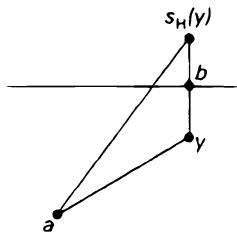
\includegraphics[keepaspectratio]{images/part001_5f5a2798.jpg}}\\
Fig. 1

\begin{enumerate}
\def\labelenumi{(\roman{enumi})}
\setcounter{enumi}{1}
\item
  Let \(\mathbf{C}'\) be a chamber and \(a' \in \mathbf{C}'\) . By what we have proved, there exists \(w \in \mathrm{W}_{\mathfrak{M}}\) such that \(w^{-1}(a') \in \overline{\mathbf{C}}\) ; hence, the chamber \(\mathbf{C}'\) meets \(\overline{w(\mathbf{C})}\) ; since \(\overline{w(\mathbf{C})}\) is the union of \(w(\mathbf{C})\) and facets with empty interior (§ 1, no. 2, Prop. 3), we have \(\mathbf{C}' = w(\mathbf{C})\) .
\item
  We have to prove that \(W = W_{\mathfrak{M}}\) and for this it suffices to prove that \(s_{H'} \in W_{\mathfrak{M}}\) for all \(H' \in \mathfrak{H}\) . Now \(H'\) is a wall of at least one chamber \(C'\) (§1, no. 4, Prop. 8); we have seen that there exists \(w \in W_{\mathfrak{M}}\) such that \(C' = w(C)\) ; consequently, there exists a wall \(H\) of \(C\) such that \(H' = w(H)\) , hence \(s_{H'} = w.s_H.w^{-1} \in W_{\mathfrak{M}}\) .
\end{enumerate}

\subsection{RELATION WITH COXETER SYSTEMS}

THEOREM 1. Let \(\mathbf{C}\) be a chamber and let \(\mathbf{S}\) be the set of reflections with respect to the walls of \(\mathbf{C}\) .

\begin{enumerate}
\def\labelenumi{(\roman{enumi})}
\item
  The pair \((\mathbf{W},\mathbf{S})\) is a Coxeter system.
\item
  Let \(w \in \mathrm{W}\) and let \(\mathrm{H}\) be a wall of \(\mathrm{C}\) . The relation \(l(s_{\mathrm{H}}w) > l(w)\) implies that the chambers \(\mathrm{C}\) and \(w(\mathrm{C})\) are on the same side of \(\mathrm{H}\) .
\item
  For any chamber \(\mathbf{C}'\) , there exists a unique element \(w \in \mathbf{W}\) such that \(w(\mathbf{C}) = \mathbf{C}'\) .
\item
  The set of hyperplanes \(\mathbf{H}\) such that \(s_{\mathrm{H}} \in \mathbf{W}\) is equal to \(\mathfrak{H}\) .
\end{enumerate}

Every element of S is of order 2 and Lemma 2 shows that S generates W. For any wall H of C, denote by \(P_{H}\) the set of elements \(w \in W\) such that the chambers C and \(w(\mathrm{C})\) (which do not meet H) are on the same side of H. We shall verify conditions \((\mathrm{A}')\) , \((\mathrm{B}')\) and (C) of Chap. IV, §1, no. 7.

\((A') 1 \in P_H\) : Trivial.

(B') \(P_{H}\) and \(s_{H}.P_{H}\) are disjoint: Indeed, \(w(\mathrm{C})\) and \(s_{H}w(\mathrm{C})\) are on opposite sides of H, so if \(w(\mathrm{C})\) is on the same side of H as C, it is not on the same side as \(s_{\mathrm{H}}w(\mathrm{C})\) .

\begin{enumerate}
\def\labelenumi{(\Alph{enumi})}
\setcounter{enumi}{2}
\tightlist
\item
  Let \(w \in \mathrm{P_H}\) and let \(\mathrm{H}'\) be a wall of \(\mathbf{C}\) such that \(ws_{\mathrm{H}'} \notin \mathrm{P_H}\) ; then \(ws_{\mathrm{H}'} = s_{\mathrm{H}}w\) : By assumption, \(w(\mathbf{C})\) is on the same side of \(\mathbf{H}\) as \(\mathbf{C}\) and \(ws_{\mathrm{H}'}(\mathbf{C})\) is on the other side. Thus, \(ws_{\mathrm{H}'}(\mathbf{C})\) and \(w(\mathbf{C})\) are on opposite sides of H; hence, the chambers \(s_{\mathrm{H}^{\prime}}(\mathrm{C})\) and C are on opposite sides of the hyperplane \(w^{-1}(\mathrm{H})\) . Let a be a point of the face of C with support \(H^{\prime}\) . The point \(a = s_{\mathrm{H}^{\prime}}(a)\) is in the closure of the two chambers C and \(s_{\mathrm{H}^{\prime}}(\mathrm{C})\) that are contained respectively in the two open half-spaces bounded by \(w^{-1}(\mathrm{H})\) ; thus, \(a \in w^{-1}(\mathrm{H})\) , so \(\mathrm{H}^{\prime} = w^{-1}(\mathrm{H})\) . From this we deduce that \(s_{\mathrm{H}^{\prime}} = w^{-1}s_{\mathrm{H}}w\) , hence \(ws_{H^{\prime}} = s_{H}w\) .
\end{enumerate}

Assertions (i) and (ii) follow from this and Prop. 6 of Chap. IV, § 1, no. 7. Moreover, we have (loc. cit., condition (A))

\[
\bigcap_ {H \in \mathfrak {M}} P _ {H} = \{1 \}.\tag{3}
\]

Lemma 2 shows that W acts transitively on the set of chambers. Moreover, if \(w \in W\) is such that \(w(\mathrm{C}) = \mathrm{C}\) , then \(w \in P_{H}\) for every wall H of C, hence w = 1 by (3). This proves (iii).

Finally, let H be a hyperplane such that \(s_{H} \in W\) . If H did not belong to H, there would be at least one chamber \(C'\) meeting H ( \(\S1\) , no. 3, Prop. 7). Every point of \(H \cap C'\) is invariant under \(s_{H}\) , and thus belongs to the chambers \(C'\) and \(s_{\mathrm{H}}(\mathrm{C}')\) ; thus, \(\mathrm{C}' = s_{\mathrm{H}}(\mathrm{C}')\) , which contradicts (iii) since \(s_{H} \neq 1\) .

COROLLARY. Let \(\Sigma\) be a set of reflections generating W. Then every reflection belonging to W is conjugate to an element of \(\Sigma\) .

Let \(\mathfrak{H}'\) be the set of hyperplanes of the form \(w(\mathrm{H})\) with \(w \in \mathrm{W}\) and \(\mathrm{H} \in \mathfrak{H}\) such that \(s_{\mathrm{H}} \in \Sigma\) . Since \(\mathrm{W}\) is generated by the family \((s_{\mathrm{H}})_{\mathrm{H} \in \mathfrak{H}'}\) and since \(\mathfrak{H}'\) is stable under \(\mathrm{W}\) , we can apply all the results of this no. to \(\mathfrak{H}'\) instead of \(\mathfrak{H}\) ; but Th. 1, (iv) shows that every reflection in \(\mathrm{W}\) is of the form \(s_{\mathrm{H}}\) with \(\mathrm{H} \in \mathfrak{H}'\) , hence the corollary.

\subsection{FUNDAMENTAL DOMAIN, STABILISERS}

Recall (Integration, Chap. VII, §2, no. 10, Def. 2) that a subset D of E is called a fundamental domain for the group W if every orbit of W in E meets D in exactly one point. This is equivalent to the following pair of conditions:

\begin{enumerate}
\def\labelenumi{\alph{enumi})}
\item
  For every \(x \in \mathrm{E}\) , there exists \(w \in \mathrm{W}\) such that \(w(x) \in \mathrm{D}\) .
\item
  If \(x, y \in D\) and \(w \in W\) are such that \(y = w(x)\) , then y = x (even though we may have \(w \neq 1\) ).
\end{enumerate}

We are going to prove the following three statements:

THEOREM 2. For any chamber C, the closure \(\overline{\mathbf{C}}\) of C is a fundamental domain for the action of W on E.

PROPOSITION 1. Let \(\mathbf{F}\) be a facet and \(\mathbf{C}\) a chamber such that \(\mathbf{F} \subset \overline{\mathbf{C}}\) . Let \(w \in W\) . The following conditions are equivalent:

\begin{enumerate}
\def\labelenumi{(\roman{enumi})}
\item
  \(w(\mathbf{F})\) meets F;
\item
  \(w(\mathbf{F}) = \mathbf{F};\)
\item
  \(w(\overline{\mathrm{F}}) = \overline{\mathrm{F}};\)
\item
  w fixes at least one point of F;
\item
  w fixes every point of F;
\item
  w fixes every point of \(\overline{\mathbf{F}}\) ;
\item
  w belongs to the subgroup of W generated by the reflections with respect to the walls of C containing F.
\end{enumerate}

For every subset A of E, denote by \(W(A)\) the subgroup of W consisting of the elements that fix every point of A.

PROPOSITION 2. Let A be a non-empty subset of E, let \(\mathfrak{H}_{\mathrm{A}}\) be the set of hyperplanes \(\mathrm{H} \in \mathfrak{H}\) containing A, let \(\mathrm{A}'\) be the intersection of the \(\mathrm{H} \in \mathfrak{H}_{\mathrm{A}}\) , and let F be a facet of E open in \(\mathrm{A}'\) (§1, no. 3, Prop. 7). Then \(\mathrm{W(A)} = \mathrm{W(A')} = \mathrm{W(F)}\) , and \(\mathrm{W(A)}\) is generated by the reflections with respect to the hyperplanes in \(\mathfrak{H}_{\mathrm{A}}\) .

We first prove the following assertion:

\begin{enumerate}
\def\labelenumi{(\Roman{enumi})}
\tightlist
\item
  Let C be a chamber, let x and y be two points of \(\overline{C}\) and let \(w \in W\) be such that \(w(x) = y\) . Then x = y and w belongs to the subgroup \(W_{N}\) , where N is the set of walls of C containing x.
\end{enumerate}

We argue by induction on the length \(q\) of \(w\) (relative to the set \(S\) of reflections with respect to the walls of \(C\) ), the case \(q = 0\) being obvious. If \(q \geqslant 1\) , there exist a wall \(H\) of \(C\) and an element \(w' \in W\) such that \(w = s_H w'\) and \(l(w') = q - 1\) . Since \(l(s_H w) < l(w)\) , the chambers \(C\) and \(w(C)\) are on opposite sides of \(H\) by Th. 1 of no. 2. Thus, \(\overline{C} \cap w(\overline{C}) \subset H\) , so \(y \in H\) . Thus \(y = w'(x)\) and the induction hypothesis implies that \(x = y\) and \(w' \in W_{\mathfrak{N}}\) . Since \(y \in H\) , it follows that \(H \in \mathfrak{N}\) , and hence that \(w = s_H w' \in W_{\mathfrak{N}}\) , completing the proof of (I).

Proof of Theorem 2: this follows from (I) and Lemma 2.

Proof of Proposition 1: we know that two distinct facets are disjoint and have distinct closures (§1, no. 2, Cor. of Prop. 3). The equivalence of (i), (ii) and (iii) follows. On the other hand, it is clear that

\[
(\mathrm{vii}) \Longrightarrow (\mathrm{vi}) \Longrightarrow (\mathrm{v}) \Longrightarrow (\mathrm{iv}) \Longrightarrow (\mathrm{i})
\]

and assertion (I) shows that (i) \(\Longrightarrow\) (vii).

Proof of Proposition 2: let \(\mathbf{A}''\) be the affine subspace of \(\mathbf{E}\) generated by A. Clearly, \(\mathrm{W(A)} = \mathrm{W(A'')}\) . By Prop. 7 of §1, no. 3, there exists a point \(x \in \mathbf{A}''\) that does not belong to any hyperplane \(\mathbf{H} \in \mathfrak{H} - \mathfrak{H}_{\mathbf{A}}\) . Let \(\mathbf{F}_x\) be the facet containing \(x\) : it is open in \(\mathbf{A}''\) and Prop. 1 shows that

\[
\mathrm{W} \left(\mathrm{F} _ {x}\right) \subset \mathrm{W} \left(\mathrm{A} ^ {\prime}\right) \subset \mathrm{W} (\mathrm{A}) = \mathrm{W} \left(\mathrm{A} ^ {\prime \prime}\right) \subset \mathrm{W} (\{x \}) = \mathrm{W} \left(\mathrm{F} _ {x}\right),
\]

hence \(\mathrm{W(A) = W(A') = W(F_x)}\) . Replacing A by F, we also have

\[
\mathrm{W} (\mathrm{A}) = \mathrm{W} (\mathrm{F}),
\]

hence the proposition.

Remarks. 1) It follows from Th. 2 that, if C is a chamber and F a facet, there exists a unique facet \(F'\) contained in \(\overline{C}\) that is transformed into F by an element of W.

\begin{enumerate}
\def\labelenumi{\arabic{enumi})}
\setcounter{enumi}{1}
\item
  It follows from Props. 1 and 2 that, for any non-empty subset A of E, there exists a point \(a \in E\) such that \(W(A) = W(\{a\})\) ; moreover, the group \(W(A)\) is a Coxeter group (Th. 1).
\item
  Let \(\mathbf{C}\) be a chamber of \(\mathbf{E}\) and \(\mathbf{S}\) the set of reflections with respect to the walls of \(\mathbf{C}\) . Let \(w \in W\) and let \((s_1, \ldots, s_q)\) be a reduced decomposition of \(w\) with respect to \(\mathbf{S}\) . If \(x \in \overline{\mathbf{C}}\) is fixed by \(w\) , then \(s_j(x) = x\) for all \(j\) : this follows from Prop. 1 above and Cor. 1 of Prop. 7 of Chap. IV, §1.
\end{enumerate}

\subsection{COXETER MATRIX AND COXETER GRAPH OF W}

Let C be a chamber, \(S = S(C)\) the set of orthogonal reflections with respect to the walls of C and \(M = (m(s, s'))\) the Coxeter matrix of the Coxeter system (W, S) (Chap. IV, §1, no. 9): recall that \(m(s, s')\) is the order (finite or infinite) of the element \(ss'\) of W (for \(s, s' \in S\) ). If \(C'\) is another chamber, the unique element \(w \in W\) such that \(w(C) = C'\) defines a bijection

\[
s \mapsto f (s) = w s w ^ {- 1}
\]

from S to \(S' = S(C')\) , and we have \(m(f(s), f(s')) = m(s, s')\) . It follows that, if W acts on the set X of pairs \((C, s)\) , where C is a chamber and \(s \in S(C)\) , by \(w.(C, s) = (w(C), wsw^{-1})\) , each orbit i of W in X meets each of the sets \(\{C\} \times S(C)\) in exactly one point, which we denote by \((C, s_i(C))\) . Thus, if I is the set of orbits and \(i, j \in I\) , the number \(m_{ij} = m(s_i(C), s_j(C))\) is independent of the choice of chamber C. The matrix \(M(W) = (m_{ij})_{i,j \in I}\) is a Coxeter matrix called the Coxeter matrix of W. The Coxeter graph associated to M(W) (Chap. IV, §1, no. 9) is called the Coxeter graph of W.

Let C be a chamber. For any \(i \in I\) , denote by \(\mathrm{H}_{i}(\mathrm{C})\) the wall of C such that \(s_{i}(\mathrm{C})\) is the reflection with respect to \(\mathrm{H}_{i}(\mathrm{C})\) and by \(e_{i}(\mathrm{C})\) the unit vector orthogonal to \(\mathrm{H}_{i}(\mathrm{C})\) on the same side of \(\mathrm{H}_{i}(\mathrm{C})\) as C. The map \(i \mapsto \mathrm{H}_{i}(\mathrm{C})\) is called the canonically indexed family of walls of C.

PROPOSITION 3. Let \(\mathbf{C}\) be a chamber and let \(i, j \in \mathbf{I}\) with \(i \neq j\) . Put \(s_i = s_i(\mathbf{C})\) , \(\mathbf{H}_i = \mathbf{H}_i(\mathbf{C})\) , \(e_i = e_i(\mathbf{C})\) and define \(s_j\) , \(\mathbf{H}_j\) and \(e_j\) similarly.

\begin{enumerate}
\def\labelenumi{(\roman{enumi})}
\item
  If \(\mathrm{H}_i\) and \(\mathrm{H}_j\) are parallel, then \(m_{ij} = \infty\) and \(e_i = -e_j\) .
\item
  If \(\mathrm{H}_i\) and \(\mathrm{H}_j\) are not parallel, then \(m_{ij}\) is finite and
\end{enumerate}

\[
\left(e _ {i} \mid e _ {j}\right) = - \cos (\pi / m _ {i j}).\tag{4}
\]

\begin{enumerate}
\def\labelenumi{(\roman{enumi})}
\setcounter{enumi}{2}
\tightlist
\item
  We have \((e_i|e_j)\leqslant 0\)
\end{enumerate}

If \(\mathrm{H}_i\) and \(\mathrm{H}_j\) are parallel, \(s_i s_j\) is a translation (§2, no. 4, Prop. 5), so \(m_{ij} = \infty\) . Moreover, either \(e_i = e_j\) or \(e_i = -e_j\) . Now, there exists a point \(a\) (resp. \(a'\) ) in the closure of C that belongs to \(\mathrm{H}_i\) (resp. \(\mathrm{H}_j\) ) but not to \(\mathrm{H}_j\) \((\text{resp. } \mathrm{H}_i)\) . Then \((a' - a|e_i) > 0\) and \((a - a'|e_j) > 0\) , which excludes the case \(e_i = e_j\) and proves (i).

Assume now that \(H_{i}\) and \(H_{j}\) are not parallel. Choose an origin \(a \in H_{i} \cap H_{j}\) and identify T with E by the bijection \(t \mapsto a + t\) . Let V be the plane orthogonal to \(H_{i} \cap H_{j}\) and passing through a. Put \(\Gamma = V \cap D_{H_{i}}(C) \cap D_{H_{j}}(C)\) (where \(D_{H}(C)\) denotes the open half-space bounded by H and containing C (§1, no. 1)) and let D (resp. \(D'\) ) be the half-line in V contained in \(H_{i} \cap V\) (resp. \(H_{j} \cap V\) ) and in the closure of \(\Gamma\) . For a suitable orientation of V, the set \(\Gamma\) is the union of the open half-lines \(\Delta\) in V such that

\[
0 <   (\widehat {\mathrm{D} , \Delta}) <   (\widehat {\mathrm{D} , \mathrm{D} ^ {\prime}}).
\]

Let \(W'\) be the subgroup of \(W\) generated by \(s_i\) and \(s_j\) . For any \(w \in W'\) , the hyperplanes \(w(H_i)\) and \(w(H_j)\) belong to \(\mathfrak{H}\) , contain \(H_i \cap H_j\) and do not meet C. It follows that they do not meet \(\Gamma\) (§1, no. 5, Prop. 10). The Cor. of Prop. 7 of §2, no. 5 thus implies (ii).

Finally, assertion (iii) follows immediately from (i) and (ii), since \(m_{ij} \geqslant 2\) for \(i \neq j\) .

Remark. Formula (4) is actually valid for all \(i, j \in I\) : in fact, \(\pi / m_{ij} = 0\) if \(m_{ij} = \infty\) , and if \(i = j\) then \(m_{ij} = 1\) and \((e_i | e_j) = 1\) .

\subsection{SYSTEMS OF VECTORS WITH NEGATIVE SCALAR PRODUCTS}

Lemma 3. Let \(q\) be a positive quadratic form on a real vector space \(V\) and let \(B\) be the associated symmetric bilinear form. Let \(a_1, \ldots, a_n\) be elements of \(V\) such that \(B(a_i, a_j) \leqslant 0\) for \(i \neq j\) .

\begin{enumerate}
\def\labelenumi{(\roman{enumi})}
\tightlist
\item
  If \(c_{1}, \ldots, c_{n}\) are real numbers such that \(q\left(\sum_{i} c_{i} a_{i}\right) = 0\) , then
\end{enumerate}

\[
q \left(\sum_ {i} | c _ {i} | a _ {i}\right) = 0.
\]

\begin{enumerate}
\def\labelenumi{(\roman{enumi})}
\setcounter{enumi}{1}
\tightlist
\item
  If \(q\) is non-degenerate and if there exists a linear form \(f\) on \(V\) such that \(f(a_i) > 0\) for all \(i\) , the vectors \(a_1, \ldots, a_n\) are linearly independent.
\end{enumerate}

The relation \(\mathrm{B}(a_i, a_j) \leqslant 0\) for \(i \neq j\) immediately implies that

\[
q \left(\sum_ {i} | c _ {i} | a _ {i}\right) \leqslant q \left(\sum_ {i} c _ {i} a _ {i}\right),
\]

hence (i). If \(q\) is non-degenerate, the relation \(\sum_{i} c_{i} a_{i} = 0\) thus implies that

\[
\sum_ {i} | c _ {i} | a _ {i} = 0;
\]

it follows that, for any linear form \(f\) on \(\mathbf{V}\) , we have \(\sum_{i}|c_i|f(a_i) = 0\) , and hence \(c_i = 0\) for all \(i\) if we also have \(f(a_i) > 0\) for all \(i\) . This proves (ii).

Lemma 4. Let \(\mathbf{Q} = (q_{ij})\) be a real, symmetric, square matrix of order \(n\) such that:

\begin{enumerate}
\def\labelenumi{\alph{enumi})}
\item
  \(q_{ij} \leqslant 0\) for \(i \neq j\) ;
\item
  there does not exist a partition of \(\{1,2,\ldots,n\}\) into two non-empty subsets I and J such that \((i,j)\in\mathrm{I}\times\mathrm{J}\) implies \(q_{ij}=0\) ;
\item
  the quadratic form \(q(x_{1},\ldots ,x_{n}) = \sum_{i,j}q_{ij}x_{i}x_{j}\) on \(\mathbf{R}^n\) is positive.
\end{enumerate}

Then:

\begin{enumerate}
\def\labelenumi{(\roman{enumi})}
\item
  The kernel \(\mathbf{N}\) of \(q\) is of dimension 0 or 1. If \(\dim \mathbf{N} = 1\) , \(\mathbf{N}\) is generated by a vector all of whose coordinates are \(> 0\) .
\item
  The smallest eigenvalue of \(\mathbf{Q}\) is of multiplicity 1 and a corresponding eigenvector has all its coordinates \(>0\) or all its coordinates \(< 0\) .
\end{enumerate}

Since \(q\) is a positive quadratic form, the kernel \(N\) of \(q\) is the set of isotropic vectors for \(q\) (Algebra, Chap. IX, §7, no. 1, Cor. of Prop. 2). Let \(a_1, \ldots, a_n\) be the canonical basis of \(\mathbf{R}^n\) . If \(\sum_{i} c_i a_i \in N\) , Lemma 3 shows that we also have \(\sum_{i} |c_i| a_i \in N\) , and hence \(\sum_{i} q_{ji}|c_i| = 0\) for all \(j\) . Let \(I\) be the set of \(i\) such that \(c_i \neq 0\) . If \(j \notin I\) , then \(q_{ji}|c_i| \leqslant 0\) for \(i \in I\) and \(q_{ji}|c_i| = 0\) for \(i \notin I\) , so \(q_{ji} = 0\) for \(j \notin I\) and \(i \in I\) . Assumption \(b)\) thus implies that either \(I = \varnothing\) or \(I = \{1, \ldots, n\}\) . Consequently, every non-zero vector in \(N\) has all its coordinates \(\neq 0\) . If \(\dim N \geqslant 2\) , the intersection of \(N\) with the hyperplane with equation \(x_i = 0\) would be of dimension \(\geqslant 1\) , contrary to what we have just shown. The preceding argument also shows that, if \(\dim N = 1\) , then \(N\) contains a vector all of whose coordinates are \(>0\) . This proves (i).

On the other hand, we know that the eigenvalues of Q are real (Algebra, Chap. IX, §7, no. 3, Prop. 5) and positive since q is positive. Let \(\lambda\) be the smallest of them. The matrix \(Q' = Q - \lambda I_n\) is then the matrix of a degenerate positive form \(q'\) and the off-diagonal elements of \(Q'\) are the same as those of Q. Consequently, \(Q'\) satisfies conditions a), b) and c) of the statement of the lemma. Since the kernel \(N'\) of \(q'\) is the eigenspace of Q corresponding to the eigenvalue \(\lambda\) , assertion (ii) follows from (i).

Lemma 5. Let \(e_1, \ldots, e_n\) be vectors generating \(T\) such that:

\(a) (e_i | e_j) \leqslant 0 \text{ for } i \neq j;\)

\begin{enumerate}
\def\labelenumi{\alph{enumi})}
\setcounter{enumi}{1}
\tightlist
\item
  there does not exist a partition of \(\{1, \ldots, n\}\) into two non-empty subsets I and J such that \((e_i|e_j) = 0\) for \(i \in I\) and \(j \in J\) .
\end{enumerate}

Then there are two possibilities:

\begin{enumerate}
\def\labelenumi{\arabic{enumi})}
\item
  \((e_1, \ldots, e_n)\) is a basis of T;
\item
  \(n = \dim T + 1\) ; there exists a family \((c_i)_{1 \leqslant i \leqslant n}\) of real numbers \(> 0\) such that \(\sum_{i} c_i e_i = 0\) , and any family \((c_i')_{1 \leqslant i \leqslant n}\) of real numbers such that \(\sum_{i} c_i' e_i = 0\) is proportional to \((c_i)_{1 \leqslant i \leqslant n}\) .
\end{enumerate}

Put \(q_{ij} = (e_i|e_j)\) . The matrix \(Q = (q_{ij})\) then satisfies the hypotheses of Lemma 4: conditions a) and b) of Lemma 4 are the same as conditions a) and b) above, and c) is satisfied since \(\sum_{i,j} q_{ij} x_i x_j = \|\sum_{i} x_i e_i\|^2\) . The kernel N of the quadratic form \(q\) on \(\mathbf{R}^n\) , with matrix \(\mathbf{Q}\) , is the set of \((c_1, \ldots, c_n) \in \mathbf{R}^n\) such that \(\sum_{i} c_i e_i = 0\) . If \(N = \{0\}\) , the \(e_i\) are linearly dependent and we are in case 1). If \(\dim N > 0\) , Lemma 4 (i) shows that we are in case 2).

Lemma 6. Let \((e_1, \ldots, e_n)\) be a basis of T such that \((e_i | e_j) \leqslant 0\) for \(i \neq j\) .

\begin{enumerate}
\def\labelenumi{(\roman{enumi})}
\item
  If \(x = \sum_{i} c_i e_i \in \mathbf{T}\) is such that \((x|e_i) \geqslant 0\) for all \(i\) , then \(c_i \geqslant 0\) for all \(i\) .
\item
  If \(x\) and \(y\) are two elements of \(\mathrm{T}\) such that \((x|e_i) \geqslant 0\) and \((y|e_i) \geqslant 0\) for all \(i\) , then \((x|y) \geqslant 0\) . If \((x|e_i) > 0\) and \((y|e_i) > 0\) for all \(i\) , then \((x|y) > 0\) .
\end{enumerate}

Under the hypotheses of (i), assume that \(c_{i} < 0\) for some \(i\) . Let \(f\) be the linear form on \(T\) defined by \(f(e_{i}) = 1\) and

\[
f \left(e _ {j}\right) = - c _ {i} / \left(\sum_ {k = 1} ^ {n} \left| c _ {k} \right|\right) \quad \text { for } j \neq i.
\]

The vectors \(-x, e_1, \ldots, e_n\) then satisfy the hypotheses of Lemma 3 (ii) (taking for \(q\) the metric form on T). We conclude that they are linearly independent, which is absurd. Hence (i). Moreover, if \(x = \sum_{i} c_i e_i \in \mathbf{T}\) and if \(y \in \mathbf{T}\) , then \((x|y) = \sum_{i} c_i (e_i | y)\) , so (ii) follows immediately from (i).

\subsection{FINITENESS THEOREMS}

Lemma 7. Let A be a set of unit vectors in T. If there exists a real number \(\lambda < 1\) such that \((a|a') \leqslant \lambda\) for \(a, a' \in \mathbf{A}\) and \(a \neq a'\) , then the set A is finite.

For \(a, a' \in A\) such that \(a \neq a'\) , we have

\[
\left\| a - a ^ {\prime} \right\| ^ {2} = 2 - 2 (a \mid a ^ {\prime}) \geqslant 2 - 2 \lambda .
\]

Now, the unit sphere S of T being compact, there exists a finite covering of S by sets of diameter \(<(2-2\lambda)^{1/2}\) and each of these sets contains at most one point of A, hence the lemma.

Denote by \(U(w)\) the automorphism of T associated to the affine map \(w \in W\) from E to itself. We have

\[
w (x + t) = w (x) + \operatorname{U} (w). t \text {for} t \in \mathrm{T} \text {and} x \in \mathrm{E}.
\]

This defines a homomorphism U from the group W to the orthogonal group of T; the kernel of U is the set of translations belonging to W.

THEOREM 3. (i) The set of walls of a chamber is finite.

\begin{enumerate}
\def\labelenumi{(\roman{enumi})}
\setcounter{enumi}{1}
\item
  The set of directions of hyperplanes belonging to \(\mathfrak{H}\) is finite.
\item
  The group U(W) is finite.
\end{enumerate}

Assertion (i) follows immediately from Prop. 3, (iii) and Lemma 7.

We prove (ii). Let \(\mathbf{C}\) be a chamber and \(\mathfrak{M}\) the set of its walls. The facets of \(\overline{\mathbf{C}}\) (relative to \(\mathfrak{H}\) ) are the same as those relative to \(\mathfrak{M}\) (§ 1, no. 4, Prop. 9).

Since M is finite, they are finite in number. Since a facet meets only finitely many hyperplanes belonging to H, the set of hyperplanes belonging to H and meeting \(\overline{C}\) is finite, hence so is the set A(C) of unit vectors in T orthogonal to some hyperplane belonging to H and meeting \(\overline{C}\) . Consequently, there exists a real number \(\lambda < 1\) such that \((a|a') \leqslant \lambda\) for \(a, a' \in A(C)\) and \(a \neq a'\) .

Let A be the set of unit vectors in T orthogonal to a hyperplane belonging to H. Let \(a, a' \in A\) with \(a \neq a'\) . If a and \(a'\) are parallel, then \(a = -a'\) and \((a|a') = -1\) . Otherwise, let \(H \in H\) (resp. \(H' \in H\) ) be such that a (resp. \(a'\) ) is orthogonal to H (resp. \(H'\) ). We have \(H \cap H' \neq \varnothing\) , and if \(x \in H \cap H'\) there exists an element \(w \in W\) such that \(x \in w(\overline{C})\) . The vectors \(U(w).a\) and \(U(w).a'\) then belong to A(C), we have

\[
(a \mid a ^ {\prime}) = (\mathrm{U} (w). a \mid \mathrm{U} (w). a ^ {\prime}) \leqslant \lambda ,
\]

and the set \(\mathbf{A}\) is finite by Lemma 7. Hence (ii).

Now let \(w \in W\) be such that \(\mathrm{U}(w).a = a\) for all \(a \in A\) . Then \(\mathrm{U}(w).t = t\) for all t belonging to the subspace of T generated by A. On the other hand, if \(t \in T\) is orthogonal to A, we have \(\mathrm{U}(s_{\mathrm{H}}).t = t\) for all \(H \in H\) , hence \(\mathrm{U}(w).t = t\) and finally \(\mathrm{U}(w) = 1\) . Since \(\mathrm{U}(w)(\mathrm{A}) = \mathrm{A}\) for all \(w \in W\) , we deduce that \(\mathrm{U}(\mathrm{W})\) is isomorphic to a group of permutations of the finite set A, hence (iii).

PROPOSITION 4. Let C be a chamber and N a set of walls of C. Let \(W_{N}\) be the subgroup of W generated by the orthogonal reflections with respect to the elements of N. For \(H \in N\) , denote by \(e_{H}\) the unit vector orthogonal to H on the same side of H as C. The following conditions are equivalent:

\begin{enumerate}
\def\labelenumi{(\roman{enumi})}
\item
  The group \(\mathbf{W}_{\mathfrak{N}}\) is finite.
\item
  There exists a point of \(\mathbf{E}\) invariant under every element of \(W_{\mathfrak{N}}\) .
\item
  The hyperplanes belonging to \(\mathfrak{N}\) have non-empty intersection.
\item
  The family of vectors \((e_{\mathrm{H}})_{\mathrm{H}\in \mathfrak{N}}\) is free in T.
\end{enumerate}

By property (D2) at the beginning of §3, the stabiliser in W of every point of E is finite, so (ii) implies (i).

Since the group \(W_{N}\) is generated by the set of reflections with respect to the hyperplanes belonging to N, the fixed points of \(W_{N}\) are the points of E belonging to every hyperplane \(H \in N\) , hence the equivalence of (ii) and (iii).

Assume that there exists a point \(a\) of \(E\) such that \(a \in H\) for all \(H \in \mathfrak{N}\) and let \(t \in T\) be such that \(a + t \in C\) . Since \((e_H | e_{H'}) \leqslant 0\) for \(H, H' \in \mathfrak{N}\) such that \(H \neq H'\) (Prop. 3), and since \((t | e_H) > 0\) for all \(H \in \mathfrak{N}\) , Lemma 3 (ii) implies that the \(e_H\) for \(H \in \mathfrak{N}\) are linearly independent. Consequently, (iii) implies (iv).

Suppose finally that the family \((e_{\mathrm{H}})_{\mathrm{H}\in\mathfrak{N}}\) is free. Let a be a point of E. For any hyperplane \(H\in N\) , there exists a real number \(c_{H}\) such that H consists of the points \(a+t\) of E with \((t|e_{\mathrm{H}})=c_{\mathrm{H}}\) . Since the family \((e_{\mathrm{H}})\) is free, there exists \(t\in T\) such that \((t|e_{\mathrm{H}})=c_{\mathrm{H}}\) for all \(H\in N\) , and the point \(a+t\) of E belongs to all the hyperplanes \(H\in N\) . Thus, (iv) implies (iii).

Remarks. 1) Since W is generated by reflections with respect to the walls of the chamber C, the preceding proposition gives a criterion for W to be finite. We shall return to this question in no. 9.

\begin{enumerate}
\def\labelenumi{\arabic{enumi})}
\setcounter{enumi}{1}
\tightlist
\item
  Let F be a finite-dimensional real affine space and G a group of automorphisms of F. For all \(g \in G\) , denote by \(U(g)\) the automorphism of the space of translations V of F associated to g. Assume that the image \(U(G)\) is a finite subgroup of \(\mathbf{GL}(V)\) ; then V has a scalar product invariant under \(U(G)\) (Integration, Chap. VII, §3, no. 1, Prop. 1). If, in addition, G acts properly on F when it is provided with the discrete topology, and if it is generated by reflections, we can apply to G the results of this paragraph.
\end{enumerate}

\subsection{DECOMPOSITION OF THE LINEAR REPRESENTATION OF W ON T}

Let I be the set of vertices of the Coxeter graph of W (no. 4) and let J be a subset of I such that no vertex in J is linked to any vertex in I-J. Let C be a chamber, s the canonical bijection from I to the set of reflections with respect to the walls of C, and let \(W_{J,C}\) be the subgroup generated by the image \(s(\mathrm{J})\) . It follows from Chap. IV, §1, no. 9, Prop. 8, that W is the direct product of the two subgroups \(W_{J,C}\) and \(W_{I-J,C}\) . Let \(C'\) be another chamber and \(s'\) the corresponding injection of I into W. We have seen (no. 4) that if \(w \in W\) transforms C into \(C'\) , then \(s'(\mathrm{i}) = ws(\mathrm{i})w^{-1}\) for \(i \in I\) . Since \(W_{J,C}\) is normal in W, it follows that \(s'(\mathrm{i}) \in W_{J,C}\) for all \(i \in J\) . We deduce that the subgroup \(W_{J,C}\) does not depend on C. We denote it simply by \(W_{J}\) from now on.

The definition of \(W_{J,C}\) clearly extends to an arbitrary subset J of I. But if there exist a vertex in J and a vertex in I-J that are linked, then \(W_{J,C}\) is not normal and depends on the choice of C.

Let \(T_{J}^{0}\) be the subspace of T consisting of the vectors invariant under every element of \(U(W_{J})\) and let \(T_{J}\) be the subspace orthogonal to \(T_{J}^{0}\) . Since \(W_{J}\) is a normal subgroup of W, it is clear that \(T_{J}^{0}\) is invariant under \(U(W)\) , and hence so is \(T_{J}\) .

PROPOSITION 5. Let \(J_{1},\ldots,J_{s}\) be the sets of vertices of the connected components of the Coxeter graph of W. For \(1\leqslant p\leqslant s\) , put

\[
\mathrm{W} _ {p} = \mathrm{W} _ {\mathrm{J} _ {p}}, \quad \mathrm{T} _ {p} = \mathrm{T} _ {\mathrm{J} _ {p}}; \quad \mathrm{T} _ {p} ^ {\prime} = \mathrm{T} _ {\mathrm{J} _ {p}} ^ {0}, \quad \text {and} \quad \mathrm{T} _ {0} = \bigcap_ {1 \leqslant p \leqslant s} \mathrm{T} _ {p} ^ {\prime}.
\]

\begin{enumerate}
\def\labelenumi{(\roman{enumi})}
\item
  The group W is the direct product of the groups \(\mathrm{W}_p\) ( \(1 \leqslant p \leqslant s\) ).
\item
  The space \(\mathbf{T}\) is the orthogonal direct sum of the subspaces \(\mathrm{T}_0, \mathrm{T}_1, \ldots, \mathrm{T}_s\) , which are all stable under \(\mathrm{U}(\mathrm{W})\) .
\item
  For all \(q\) such that \(1 \leqslant q \leqslant s\) , the subspace \(\mathrm{T}_q'\) of \(\mathrm{T}\) consists of the vectors invariant under \(\mathrm{U}(\mathrm{W}_q)\) ; it is the direct sum of the \(\mathrm{T}_p\) for \(1 \leqslant p \leqslant s\) and \(p \neq q\) .
\item
  Let \(\mathbf{C}\) be a chamber. The subspace \(\mathrm{T}_p\) (for \(1 \leqslant p \leqslant s\) ) is generated by the vectors \(e_i(\mathbf{C})\) for \(i \in \mathrm{J}_p\) (in the notation of no. 4).
\item
  The representations of W in the subspaces \(T_{p}\) ( \(1 \leqslant p \leqslant s\) ) are absolutely irreducible, non-trivial, and pairwise inequivalent.
\end{enumerate}

Assertion (i) follows from Chap. IV, §1, no. 9. On the other hand, we have already seen that the subspaces \(\mathrm{T}_p\) are invariant under \(\mathrm{U}(\mathrm{W})\) , and so is \(\mathrm{T}_0\) . Let \(\mathrm{C}\) be a chamber; since \(\mathrm{W}_p\) is generated by the reflections \(s_i(\mathrm{C})\) for \(i \in \mathrm{J}_p\) , it is clear that \(\mathrm{T}_p'\) is the subspace orthogonal to the \(e_i(\mathrm{C})\) for \(i \in \mathrm{J}_p\) , hence (iv). Moreover, if \(i \in \mathrm{J}_p\) , \(j \in \mathrm{J}_q\) with \(p \neq q\) , then \(m_{ij} = 2\) since \(\{i,j\}\) is not an edge of the Coxeter graph of \(\mathrm{W}\) , so \((e_i|e_j) = 0\) . Assertion (ii) is now immediate. And assertion (iii) follows, since \(\mathrm{T}_q'\) is the orthogonal complement of \(\mathrm{T}_q\) .

Finally, let V be a subspace of \(T_{p}\) invariant under \(\mathrm{U}(\mathrm{W}_{p})\) . For all \(i \in J_{p}\) , either \(e_{i} \in V\) or \(e_{i}\) is orthogonal to V ( \(\S2\) , no. 2, Prop. 3). Let A (resp. B) be the set of \(i \in J_{p}\) such that \(e_{i} \in V\) (resp. \(e_{i}\) is orthogonal to V). Clearly \((e_{i}|e_{j}) = 0\) for \(i \in A\) and \(j \in B\) , and since \(J_{p}\) is connected, it follows that either A = \(\varnothing\) and V = \(\{0\}\) , or A = \(J_{p}\) and V = \(T_{p}\) . Consequently, the representation of \(W_{p}\) on \(T_{p}\) is irreducible, hence absolutely irreducible ( \(\S2\) , no. 1, Prop. 1). It is non-trivial by the very definition of \(T_{p}\) . Finally, the last assertion in (v) follows immediately from (iii).

If the subspace \(T_{0}\) of vectors in T invariant under U(W) reduces to \(\{0\}\) , then W is said to be essential; if the representation U of W on T is irreducible, then W is said to be irreducible.

COROLLARY. Assume that \(W \neq \{1\}\) . Then W is irreducible if and only if it is essential and its Coxeter graph is connected.

Remark. Under the hypotheses of Prop. 5, the subspaces \(T_{p}\) for \(0 \leqslant p \leqslant s\) are the isotypical components of the linear representation U of W on T (Algebra, Chap. VIII, §3, no. 4). It follows (loc. cit., Prop. 11) that every vector subspace V of T stable under W is the direct sum of the subspaces \(V \cap T_{p}\) for \(0 \leqslant p \leqslant s\) ; moreover (loc. cit., Prop. 10), every endomorphism commuting with the operators \(U(w)\) for \(w \in W\) leaves stable each of the \(T_{p}\) for \(0 \leqslant p \leqslant s\) and induces on them a homothety for \(1 \leqslant p \leqslant s\) . In particular, the bilinear forms \(\Phi\) on T invariant under W are the bilinear forms given by

\[
\varPhi \left(\sum_ {k} t _ {k}, \sum_ {k} t _ {k} ^ {\prime}\right) = \varPhi_ {0} (t _ {0}, t _ {0} ^ {\prime}) + \sum_ {1 \leqslant p \leqslant s} a _ {p} (t _ {p} | t _ {p} ^ {\prime}),
\]

where \(\Phi_{0}\) is a bilinear form on \(T_{0}\) and \(a_{p}\) (for \(1 \leqslant p \leqslant s\) ) is a real number: indeed, such a form \(\Phi\) can be written uniquely in the form \((t, t') \mapsto (\mathrm{A}(t)|t')\) , where A is an endomorphism of T commuting with the \(\mathrm{U}(w)\) for \(w \in W\) .
